% this file is encoded in utf-8
% v1.7

\documentclass[12pt, a4paper]{ntust_report} 

\usepackage{fontspec}   %加這個就可以設定字體 
\usepackage{xeCJK}       %讓中英文字體分開設置 
\setmainfont[Mapping=tex-text]{Times New Roman}            %設定主要字型,也就是英文字型 
\setCJKmainfont{標楷體}     %設定中文字型 
\XeTeXlinebreaklocale "zh"                %這兩行一定要加,中文才能自動換行 
\XeTeXlinebreakskip = 0pt plus 1pt       %這兩行一定要加,中文才能自動換行




% 除非校方修改了論文格式 (margins, header, footer, 浮水印)
% 或者需要增加所用的 LaTeX 套件,
% 或者要改預設中文字型、編碼
% 否則毋須修改本檔內容
% 論文撰寫,請修改以 my_  開頭檔名的各檔案



\usepackage{titletoc}
\usepackage[nospace]{cite}  % for smart citation
\usepackage{geometry}  % for easy margin settings
\usepackage{subfigure}  % for subfigure
\usepackage{multirow}
%\usepackage[dvipdfm]{graphicx}  % for graphic   using eps
\usepackage{graphicx}  % for graphic   using eps

%\usepackage{epstopdf} % 當使用pdflatex時打開,如使用latex則不需開啟,此功能為將xxx.eps 自動判讀為XXX.pdf

%\usepackage{subfig} 
\usepackage{algorithmic}  %演算法使用
\usepackage{algorithm}

%
% margins setting
\geometry{verbose,a4paper,tmargin=3.5cm,bmargin=2cm,lmargin=3cm,rmargin=3cm}
%
\usepackage{amsmath} % 各式 AMS 數學功能
\usepackage{amssymb} % 各式 AMS 數學符號
\usepackage{mathrsfs} %草寫體數學符號,在數學模式裡用 \mathscr{E} 得草寫 E
\usepackage{listings} % 程式列表套件
%
% listing setting
\lstset{breaklines=true,% 過長的程式行可斷行
extendedchars=false,% 中文處理不需要 extendedchars
texcl=true,% 中文註解需要有 TeX 處理過的 comment line, 所以設成 true
comment=[l]\%\%,% 以雙「百分號」做為程式中文註解的起頭標記,配合 MATLAB
basicstyle=\small,% 小號字體, 約 10 pt 大小
commentstyle=\upshape,% 預設是斜體字,會影響註解裏的英文,改用正體
%language=Octave % 會將一些 octave 指令以粗體顯示
}

\usepackage{url} % 在文稿中引用網址,可以用 \url{http://www.ntust.edu.tw} 方式

% 插圖套件 graphicx
% 使用者工作流程是用 pdftex 還是 latex + dvipdfmx?
% 視情況而有不同的參數
% 這裡作自動判斷
% 參考自
% http://www.tex.ac.uk/cgi-bin/texfaq2html?label=ifpdf
%\newcommand\mydvipdfmxflow{dvipdfmx}
%\newcommand\mypdftexflow{pdftex}
%
%\ifx\pdfoutput\undefined
%  % not running pdftex
%  \usepackage[dvipdfm]{graphicx}
%  \newcommand\myworkflow{dvipdfmx}  % set the flag for hyperref
%\else
%  \ifx\pdfoutput\relax
%    % not running pdftex
%    \usepackage[dvipdfm]{graphicx}
%    \newcommand\myworkflow{dvipdfmx}  % set the flag
%  \else
%    % running pdftex, with...
%    \ifnum\pdfoutput>0
%      % ... PDF output
%      \usepackage[pdftex]{graphicx}
%      \newcommand\myworkflow{pdftex}  % set the flag
%    \else
%      %...DVI output
%      \usepackage[dvipdfm]{graphicx}
%      \newcommand\myworkflow{dvipdfmx}  % set the flag
%    \fi
%  \fi
%\fi

\usepackage{fancyhdr}  % 借用增強功能型 header 套件來擺放浮水印 
% (佔用了 central header)
% 不需要浮水印的使用者仍可利用此套件,產生所需的 header, footer
%
% 啟動 fancy header/footer 套件
\pagestyle{fancy}
\fancyhead{}  % reset left, central, right header to empty
\fancyfoot[C]{\thepage} %中間 footer 擺放頁碼
\renewcommand{\headrulewidth}{0pt} % header 的直線; 0pt 則無線

% 如果不需要任何浮水印,則請把下列介於 >>> 與 <<< 之間
% 的文字行關掉 (行首加上百分號)
%% 浮水印 >>> 
%7/23
%
% this file is encoded in utf-8
% v1.7
% 如果浮水印不是全篇需要,請把下列介於 >>> 與 <<<
% 的「全篇浮水印專用碼」關掉 (行首加百分號)
% 參考自 Keith Reckdahl 寫的 "Using Imported Graphics in LATEX2e" (epslatex.pdf) p.39
% 如果只有特定頁需要浮水印
% 則依該頁屬性使用下列之一的命令 
% 普通頁命令 \thispagestyle{WaterMarkPage}
% plain 頁命令 \thispagestyle{PlainWaterMarkPage}
% empty 頁命令 \thispagestyle{EmptyWaterMarkPage}


% 將重複使用的浮水印章
% 圖檔是 my_watermark.xxx
% 副檔名可以不加,可以是 latex 系統能處裡的任何格式:pdf, gif, png, jpg, eps, ...
% 某些圖檔格式在某些工作流程可能需要作前置處裡。
% 例如,pdflatex 無法直接處理 eps 檔
%  latex + dvipdfmx 無法直接處理 pdf, gif, png, jpg, 需要用 ebb 小工具程式
%  對圖檔產生 .bb 對應檔。
% old code
%\newsavebox{\mywatermark}
%\sbox{\mywatermark}{\includegraphics[keepaspectratio,%
%height=0.8\textheight,%
%width=0.8\textwidth]{my_watermark}}
% new code
\newsavebox{\mywatermark}
%7/23
\sbox{\mywatermark}{
\includegraphics[keepaspectratio,
width=2.5cm]{watermark/ntust_watermark.eps}}


% 將 central header 擺放浮水印的巨集指令
\newcommand{\PlaceWaterMark}{\fancyhead[C]{\setlength{\unitlength}{1in}%
\begin{picture}(0,0)%
%\put(-2.2,-6){\usebox{\mywatermark}}% old code
\put(-0.5,-5.3){\usebox{\mywatermark}}% new code
\end{picture}}%
}

\fancyhead{}  % reset left, central, right header to empty
%% 如果不需整篇論文都要浮水印
%% 則下面  >>> 與 <<< 之間的程式碼請關閉
%% >>> 全篇浮水印

\PlaceWaterMark  % 每一頁都有浮水印 (除了 plain、empty 頁以外)

% 重新定義 plain 頁面
% 每張 plain 頁面 (每一章的第一頁) 也加浮水印

\fancypagestyle{plain}{%
\fancyhead{}%
\PlaceWaterMark%
\fancyfoot{}%
\fancyfoot[C]{\thepage}
\renewcommand{\headrulewidth}{0pt}%
\renewcommand{\footrulewidth}{0pt}%
}
%% <<< 全篇浮水印

%% 如果只有一、兩頁需要有浮水印
%% 可以在該頁 (有頁碼) 使用 \thispagestyle{WaterMarkPage}
%% 此命令不影響原有的 header、footer
\fancypagestyle{WaterMarkPage}{%
\PlaceWaterMark%
}

%% 如果只有一、兩頁 plain 頁需要有浮水印 (如 摘要、自傳等)
%% 可以在該頁 (有頁碼) 使用 \thispagestyle{PlainWaterMarkPage}
%% 只有頁碼與浮水印,沒有其他的 header、footer
%% 等同於 plain page style + water mark
\fancypagestyle{PlainWaterMarkPage}{%
\fancyhead{}%
\PlaceWaterMark%
\fancyfoot{}%
\fancyfoot[C]{\thepage}
\renewcommand{\headrulewidth}{0pt}%
\renewcommand{\footrulewidth}{0pt}%
}

%% 如果只有一、兩頁 empty 頁需要有浮水印 (如封面、書名頁)
%% 可以在該頁 (無頁碼) 使用 \thispagestyle{EmptyWaterMarkPage}
%% 等同於 empty page style + water mark
\fancypagestyle{EmptyWaterMarkPage}{%
\fancyhead{}%
\PlaceWaterMark%
\fancyfoot{}%
\renewcommand{\headrulewidth}{0pt}%
\renewcommand{\footrulewidth}{0pt}%
}

\fancypagestyle{AppendixPage}{%
\fancyhead{}%
\fancyfoot{}%
\fancyfoot[C]{\thepage}
\renewcommand{\headrulewidth}{0pt}%
\renewcommand{\footrulewidth}{0pt}%
}
%% <<< 浮水印



% global page layout
\newcommand{\mybaselinestretch}{1.5}  %行距 1.5 倍 + 20%, (約為 double space)
\renewcommand{\baselinestretch}{\mybaselinestretch}  % 論文行距預設值
\parskip=2ex  % 段落之間的間隔為兩個 x 的高度
\parindent = 24Pt  % 段首內縮由 CJK 控制,所以這裡就設成不內縮

%%%%%%%%%%%%%%%%%%%%%%%%%%%%%
%  end of preamble
%%%%%%%%%%%%%%%%%%%%%%%%%%%%%  %基本的環境設定  無需改變  

\begin{document}


	% 下列中文名詞的定義,如果以註解方式關閉取消,
% 則會以系統原先的預設值 (英文) 替代
% 名詞 \prechaptername 預設值為 Chapter
% 名詞 \postchaptername 預設值為空字串
% 名詞 \tablename 預設值為 Table
% 名詞 \figurename 預設值為 Figure

\renewcommand\prechaptername{第} % 出現在每一章的開頭的「第 x 章」
\renewcommand\postchaptername{章}
\renewcommand{\tablename}{表} % 在文章中 table caption 會以「表 x」表示
\renewcommand{\figurename}{圖} % 在文章中 figure caption 會以「圖 x」表示

% 下列中文名詞的定義,用於論文固定的各部分之命名 (出現於目錄與該頁標題)
\newcommand{\nameInnerCover}{教授推薦書}
\newcommand{\nameCommitteeForm}{論文口試委員審定書}
\newcommand{\nameCopyrightForm}{授權書}
\newcommand{\nameCabstract}{論文摘要}
\newcommand{\nameEabstract}{Abstract}
\newcommand{\nameAckn}{誌謝}
\newcommand{\nameToc}{目錄}
\newcommand{\nameLot}{表目錄}
\newcommand{\nameTof}{圖目錄}
\newcommand{\nameToa}{演算法目錄}
\newcommand{\nameSlist}{符號說明}
\newcommand{\nameRef}{參考文獻}
\newcommand{\nameVita}{自傳}
 %在此檔案處定義文章中的中文名詞

	%----------------------------------------------------------------------------------------------------------------------------------------------------------
	%%% 以下是載入前頁、本文、後頁
	% 此行請勿更動

	%----------------------------------------------------------------------------------------------------------------------------------------------------------
	% front matter 前頁
	% 包括封面、書名頁、中文摘要、英文摘要、誌謝、目錄、表目錄、圖目錄、符號說明
	% 在撰寫各章草稿時,可以把此部份「關掉」,以節省無謂的編譯時間。
	% 實際內容由
	%    my_names.tex, my_cabstract.tex, my_eabstract.tex, my_ackn.tex, my_symbols.tex
	% 決定
	% ntust_frontpages.tex 此檔只提供整體架構的定義,不需更動
	% 在撰寫各章草稿時,可以把此部份「關掉」,以節省無謂的編譯時間。
	
	%
% this file is encoded in utf-8
% v1.7
% do not change the content of this file
% unless the thesis layout rule is changed
% 無須修改本檔內容,除非校方修改了
% 封面、書名頁、中文摘要、英文摘要、誌謝、目錄、表目錄、圖目錄、符號說明
% 等頁之格式
% this file is encoded in utf-8
%v1.7

% make the line spacing in effect
\renewcommand{\baselinestretch}{\mybaselinestretch}
\large % it needs a font size changing command to be effective

% default variables definitions
% 注意!!此處只是預設值,不需更改此處
% 請更改 my_names.tex 內容
\newcommand\cTitle{論文題目}
\newcommand\eTitle{MY THESIS TITLE}
\newcommand\myCname{王鐵雄}
\newcommand\myEname{Aron Wang}
\newcommand\myStudentID{M9315048}
\newcommand\advisorCnameA{南宮明博士}
\newcommand\advisorEnameA{Dr.~Ming Nangong}
\newcommand\advisorCnameB{李斯坦博士}
\newcommand\advisorEnameB{Dr.~Stein Lee}
\newcommand\advisorCnameC{徐 石博士}
\newcommand\advisorEnameC{Dr.~Sean~Hsu}
\newcommand\univCname{國立台灣科技大學}
\newcommand\univEname{National Taiwan University of science and technology}
\newcommand\deptCname{光電工程研究所}
\newcommand\fulldeptEname{Graduate School of Electro-Optical Engineering}
\newcommand\deptEname{Electro-optical Engineering}
\newcommand\collEname{College of Engineering}
\newcommand\degreeCname{碩士}
\newcommand\degreeEname{Master of Science}
\newcommand\cYear{九十四}
\newcommand\cMonth{六}
\newcommand\cDay{十}
%\newcounter{eYear}
\newcommand\eYear{2006}
\newcommand\eMonth{June}
\newcommand\ePlace{Chungli, Taoyuan, Taiwan}


 % user's names; to replace those default variable definitions
%
% this file is encoded in utf-8
% v1.7
% 填入你的論文題目、姓名等資料
% 如果題目內有必須以數學模式表示的符號,請用 \mbox{} 包住數學模式,如下範例
% 如果中文名字是單名,與姓氏之間建議以全形空白填入,如下範例
% 英文名字中的稱謂,如 Prof. 以及 Dr.,其句點之後請以不斷行空白~代替一般空白,如下範例
% 如果你的指導教授沒有如預設的三位這麼多,則請把相對應的多餘教授的中文、英文名
%    的定義以空的大括號表示
%    如,\renewcommand\advisorCnameB{}
%          \renewcommand\advisorEnameB{}
%          \renewcommand\advisorCnameC{}
%          \renewcommand\advisorEnameC{}

% 論文題目 (中文)
\renewcommand\cTitle{%我的碩士論文題目 
校舍耐震資料庫之資料探勘
}

% 論文題目 (英文)
\renewcommand\eTitle{%My Thesis Title  
Data Mining on Aseismic School Building Database 
%My Thesis Title  \mbox{$\cal{H}_\infty$} and \mbox{Al$_x$Ga$_{1-x}$As}
}

% 我的姓名 (中文)
\renewcommand\myCname{高偉格}

% 我的姓名 (英文)
\renewcommand\myEname{Kao, Wei-Ko}

%我的學號
\renewcommand\myStudentID{D9505501}

% 指導教授A的姓名 (中文)
\renewcommand\advisorCnameA{陳鴻銘 博士}

% 指導教授A的姓名 (英文)
\renewcommand\advisorEnameA{Dr. Hung-Ming Cheng}

% 指導教授B的姓名 (中文)
\renewcommand\advisorCnameB{}

% 指導教授B的姓名 (英文)
\renewcommand\advisorEnameB{}

% 指導教授C的姓名 (中文)
\renewcommand\advisorCnameC{}

% 指導教授C的姓名 (英文)
\renewcommand\advisorEnameC{}

% 校名 (中文)
\renewcommand\univCname{國立台灣科技大學}

% 校名 (英文)
%\renewcommand\univEname{National Taiwan University of science and technology}

% 系所名 (中文)
\renewcommand\deptCname{營~建~工~程~系}

% 系所全名 (英文)
%\renewcommand\fulldeptEname{Graduate School of Electro-Optical Engineering}

% 系所短名 (英文, 用於書名頁學位名領域)
%\renewcommand\deptEname{Electro-Optical Engineering}

% 學院英文名 (如無,則以空的大括號表示)
%\renewcommand\collEname{College of Electrical and Communication Engineering}

% 學位名 (中文)
\renewcommand\degreeCname{博士學位}

% 學位名 (英文)
%\renewcommand\degreeEname{Master of Science}

% 口試年份 (中文、民國)
\renewcommand\cYear{一零二}

% 口試月份 (中文)
\renewcommand\cMonth{七} 

% 口試月份 (中文)
\renewcommand\cDay{七} 

% 口試年份 (阿拉伯數字、西元)
%\renewcommand\eYear{2009} 

% 口試月份 (英文)
%\renewcommand\eMonth{July}

% 學校所在地 (英文)
%\renewcommand\ePlace{Taipei, Taiwan}

%畢業級別;用於書背列印;若無此需要可忽略
\newcommand\GraduationClass{95}

%%%%%%%%%%%%%%%%%%%%%%
\newcommand\itsempty{}
%%%%%%%%%%%%%%%%%%%%%%%%%%%%%%%
%       ntust cover 封面
%%%%%%%%%%%%%%%%%%%%%%%%%%%%%%%
%
\begin{titlepage}
% no page number
% next page will be page 1

% aligned to the center of the page
\begin{center}
% font size (relative to 12 pt):
% \large (14pt) < \Large (18pt) < \LARGE (20pt) < \huge (24pt)< \Huge (24 pt)
%



\begin{figure}[htbp]
	\begin{minipage}[t]{5cm} 
		\raggedright
		
\includegraphics[width=1.1in]{frontpages/ntust_logo.eps}
		\label{fig:ntust_logo}
		\vspace{0.5cm}
	\end{minipage}% 
	\begin{minipage}[b]{0.5\textwidth} 
	\centering
	\makebox[3cm][c]{\Huge{\univCname}}\\  %顯示中文校名
	\vspace{0.5cm}
	\makebox[3cm][c]{\Huge{\deptCname}}\\ %顯示中文系所名
	\vspace{0.5cm}
	\makebox[3cm][c]{\Huge{\degreeCname 論文}}\\ %顯示論文種類 (中文)
	\vspace{0.5cm}
	\end{minipage}%
\\ 
\rule{16cm}{3pt}
\end{figure}
%\hfill


%\makebox[8cm][s]{\textbf{\Huge{\degreeCname 論文(初稿)}}}\\ %顯示論文種類 (中文)
\vspace{1cm}
%
% Set the line spacing to single for the titles (to compress the lines)
\renewcommand{\baselinestretch}{1}   %行距 1 倍
%\large % it needs a font size changing command to be effective
\textbf{\LARGE{\cTitle}}\\  % 中文題目
%
\vspace{1cm}
%
\Large{\eTitle}\\ %英文題目
\vspace{5cm}
% \makebox is a text box with specified width;
% option s: stretch
% use \makebox to make sure
% 「研究生:」 與「指導教授:」occupy the same width
\hspace{4.5cm} \makebox[3cm][s]{\Large{研 究 生:}}
\Large{\myCname}  % 顯示作者中文名
\hfill \makebox[1cm][s]{}\\
%
\vspace{0.3cm}
\hspace{4.5cm} \makebox[3cm][s]{\Large{學號:}}
\Large{\myStudentID}  %顯示指導教授A中文名
\hfill \makebox[1cm][s]{}\\
%
\vspace{1cm}
\hspace{4.5cm} \makebox[3cm][s]{\Large{指導教授:}}
\Large{\advisorCnameA}  %顯示指導教授A中文名
\hfill \makebox[1cm][s]{}\\
%
% 判斷是否有共同指導的教授 B
\ifx \advisorCnameB  \itsempty
\relax % 沒有 B 教授,所以不佔版面,不印任何空白
\else
% 共同指導的教授 B
\hspace{4.5cm} \makebox[3cm][s]{}
\Large{\advisorCnameB}  %顯示指導教授B中文名
\hfill \makebox[1cm][s]{}\\
\fi
%
% 判斷是否有共同指導的教授 C
\ifx \advisorCnameC  \itsempty
\relax % 沒有 C 教授,所以不佔版面,不印任何空白
\else
% 共同指導的教授 C
\hspace{4.5cm} \makebox[3cm][s]{}
\Large{\advisorCnameC}  %顯示指導教授C中文名
\hfill \makebox[1cm][s]{}\\
\fi
%
\vfill
\makebox[10cm][s]{\Large{中華民國\cYear 年\cMonth 月\cDay 日}}%
%
\end{center}
% Resume the line spacing to the desired setting
\renewcommand{\baselinestretch}{\mybaselinestretch}   %恢復原設定
% it needs a font size changing command to be effective
% restore the font size to normal
\normalsize
\end{titlepage}
%%%%%%%%%%%%%%

%% 從摘要到本文之前的部份以小寫羅馬數字印頁碼
% 但是從「書名頁」(但不印頁碼) 就開始計算
%\setcounter{page}{1}
\pagenumbering{Roman}
%\pagenumbering{arabic}
%%%%%%%%%%%%%%%%%%%%%%%%%%%%%%%
%       指導教授推薦書 
%%%%%%%%%%%%%%%%%%%%%%%%%%%%%%%
%
% insert the printed standard form when the thesis is ready to bind
% 在口試完成後,再將已簽名的推薦書放入以便裝訂
% create an entry in table of contents for 推薦書
% 目前送出空白頁
%\newpage{\thispagestyle{empty}\addcontentsline{toc}{chapter}{\nameInnerCover}\mbox{}\clearpage}%
%\newpage

% 判斷是否要浮水印?
\ifx\mywatermark\undefined 
  \thispagestyle{empty}  % 無頁碼、無 header (無浮水印)
\else
  \thispagestyle{EmptyWaterMarkPage} % 無頁碼、有浮水印
\fi

%%%%%%%%%%%%%%%%%%%%%%%%%%%%%%%%%%%%%%%%%%%%%%%%%%%%%%%%%%%%%%%
%%no page number
%% create an entry in table of contents for 書名頁
%\addcontentsline{toc}{chapter}{\nameInnerCover}
%
%
%% aligned to the center of the page
%\begin{center}
%% font size (relative to 12 pt):
%% \large (14pt) < \Large (18pt) < \LARGE (20pt) < \huge (24pt)< \Huge (24 pt)
%% Set the line spacing to single for the titles (to compress the lines)
%\renewcommand{\baselinestretch}{1}   %行距 1 倍
%% it needs a font size changing command to be effective
%%中文題目
%\Large{\cTitle}\\ %%%%%
%\vspace{1cm}
%% 英文題目
%\Large{\eTitle}\\ %%%%%
%%\vspace{1cm}
%\vfill
%% \makebox is a text box with specified width;
%% option s: stretch
%% use \makebox to make sure
%% 「研究生:」 與「指導教授:」occupy the same width
%\makebox[3cm][s]{\large{研 究 生:}}
%\makebox[3cm][l]{\large{\myCname}} %%%%%
%\hfill
%\makebox[2cm][s]{\large{Student: }}
%\makebox[5cm][l]{\large{\myEname}}\\ %%%%%
%%
%%\vspace{1cm}
%%
%\makebox[3cm][s]{\large{指導教授:}}
%\makebox[3cm][l]{\large{\advisorCnameA}} %%%%%
%\hfill
%\makebox[2cm][s]{\large{Advisor: }}
%\makebox[5cm][l]{\large{\advisorEnameA}}\\ %%%%%
%%
%% 判斷是否有共同指導的教授 B
%\ifx \advisorCnameB  \itsempty
%\relax % 沒有 B 教授,所以不佔版面,不印任何空白
%\else
%%共同指導的教授B
%\makebox[3cm][s]{}
%\makebox[3cm][l]{\large{\advisorCnameB}} %%%%%
%\hfill
%\makebox[2cm][s]{}
%\makebox[5cm][l]{\large{\advisorEnameB}}\\ %%%%%
%\fi
%%
%% 判斷是否有共同指導的教授 C
%\ifx \advisorCnameC  \itsempty
%\relax % 沒有 C 教授,所以不佔版面,不印任何空白
%\else
%%共同指導的教授C
%\makebox[3cm][s]{}
%\makebox[3cm][l]{\large{\advisorCnameC}} %%%%%
%\hfill
%\makebox[2cm][s]{}
%\makebox[5cm][l]{\large{\advisorEnameC}}\\ %%%%%
%\fi
%%
%% Resume the line spacing to the desired setting
%\renewcommand{\baselinestretch}{\mybaselinestretch}   %恢復原設定
%\large %it needs a font size changing command to be effective
%%
%\vfill
%\makebox[4cm][s]{\large{\univCname}}\\% 校名
%\makebox[6cm][s]{\large{\deptCname}}\\% 系所名
%\makebox[3cm][s]{\large{\degreeCname 論文}}\\% 學位名
%%
%%\vspace{1cm}
%\vfill
%\large{A Thesis}\\%
%\large{Submitted to }%
%%
%\large{\fulldeptEname}\\%系所全名 (英文)
%%
%%
%\ifx \collEname  \itsempty
%\relax % 沒有學院名 (英文),所以不佔版面,不印任何空白
%\else
%% 有學院名 (英文)
%\large{\collEname}\\% 學院名 (英文)
%\fi
%%
%\large{\univEname}\\%校名 (英文)
%%
%\large{in Partial Fulfillment of the Requirements}\\
%%
%\large{for the Degree of}\\
%%
%\large{\degreeEname}\\%學位名(英文)
%
%\large{in}\\
%%
%\large{\deptEname}\\%系所短名(英文;表明學位領域)
%%
%\large{\eMonth\ \eYear}\\%月、年 (英文)
%%
%\large{\ePlace}% 學校所在地 (英文)
%\vfill
%\large{中華民國}%
%\large{\cYear}% %%%%%
%\large{年}%
%\large{\cMonth}% %%%%%
%\large{月}\\
%\end{center}
%% restore the font size to normal
%\normalsize
%\clearpage


%%%%%%%%%%%%%%%%%%%%%%%%%%%%%%%%%%%%%%%%%%%%%%%%%%%%%%%%%%%%%%%%%%%%%
%%%%%%%%%%%%%%%%%%%%%%%%%%%%%%%
%       論文口試委員審定書 (計頁碼,但不印頁碼) 
%%%%%%%%%%%%%%%%%%%%%%%%%%%%%%%
%
% insert the printed standard form when the thesis is ready to bind
% 在口試完成後,再將已簽名的審定書放入以便裝訂
% create an entry in table of contents for 審定書
% 目前送出空白頁

%\newpage{\thispagestyle{empty}\addcontentsline{toc}{chapter}{\nameCommitteeForm}\mbox{}\clearpage}%


%%%%%%%%%%%%%%%%%%%%%%%%%%%%%%%
%       中文摘要 
%%%%%%%%%%%%%%%%%%%%%%%%%%%%%%%
%
\newpage
\thispagestyle{plain}  % 無 header,但在浮水印模式下會有浮水印
% create an entry in table of contents for 中文摘要
\addcontentsline{toc}{chapter}{\nameCabstract}

% aligned to the center of the page
\begin{center}
% font size (relative to 12 pt):
% \large (14pt) < \Large (18pt) < \LARGE (20pt) < \huge (24pt)< \Huge (24 pt)
% Set the line spacing to single for the names (to compress the lines)
\renewcommand{\baselinestretch}{1}   %行距 1 倍
% it needs a font size changing command to be effective
%\large{\cTitle}\\  %中文題目
%\vspace{0.83cm}
% \makebox is a text box with specified width;
% option s: stretch
% use \makebox to make sure
% each text field occupies the same width
%\makebox[1.5cm][s]{\large{學生:}}
%\makebox[3cm][l]{\large{\myCname}} %學生中文姓名
%\hfill
%
%\makebox[3cm][s]{\large{指導教授:}}
%\makebox[3cm][l]{\large{\advisorCnameA}} \\ %教授A中文姓名
%
% 判斷是否有共同指導的教授 B
\ifx \advisorCnameB  \itsempty
\relax % 沒有 B 教授,所以不佔版面,不印任何空白
\else
%共同指導的教授B
\makebox[1.5cm][s]{}
\makebox[3cm][l]{} %%%%%
\hfill
\makebox[3cm][s]{}
\makebox[3cm][l]{\large{\advisorCnameB}}\\ %教授B中文姓名
\fi
%
% 判斷是否有共同指導的教授 C
\ifx \advisorCnameC  \itsempty
\relax % 沒有 C 教授,所以不佔版面,不印任何空白
\else
%共同指導的教授C
\makebox[1.5cm][s]{}
\makebox[3cm][l]{} %%%%%
\hfill
\makebox[3cm][s]{}
\makebox[3cm][l]{\large{\advisorCnameC}}\\ %教授C中文姓名
\fi
%
%\vspace{0.42cm} %2013/06/06
\vspace{0.38cm}
%
%\large{\univCname}\large{\deptCname}\\ %校名系所名
%\vspace{0.83cm}
%\vfill
\makebox[2.5cm][s]{\LARGE{中文摘要}}\\
\end{center}
% Resume the line spacing to the desired setting
\renewcommand{\baselinestretch}{\mybaselinestretch}   %恢復原設定
%it needs a font size changing command to be effective
% restore the font size to normal
\normalsize
%%%%%%%%%%%%%

台灣國家實驗研究院地震工程研究中心(NCREE)在九二一大地震後,與教育部合作執行加速國中小老舊校舍及相關設備補強整建計畫,評估全台灣的各級學校校舍之耐震能力,在此計畫執行的過程中產生了大量的評估與調查資料,因此 NCREE 便建立了一個校舍耐震能力資料庫來收集各種相關的資料,收集了包括校舍的各種設計參數、材料強度、校舍現況及年齡、技師的評估與補強建議方案、實際補強的金額與補強方法等。此一資料庫所收集的校舍資料數量龐大,除了當初設計的目的之外,應該還潛藏難以由人直接判斷取得的知識(knowledge)、模式(pattern),而資料探勘(Data Mining)就是用來分析這種數量龐大的資料,可以從中找出潛藏知識的相關技術的統稱,本研究之目的即為利用資料探勘技術來發掘潛藏於此校舍耐震資料庫中的知識,並從資料探勘的四種主要分析方法:回歸、分類、分群、關聯出發,分別探討各種方法在此資料庫中有何可能的分析方向,有哪些可能的潛藏知識,並進行分析,最後得到了三個有用且可靠度足夠的關係模型,分別為校舍資訊與耐震能力之關係模型、校校舍資訊與破壞構件之關係模型以及校舍資訊與補強經費之關係模型。
	

%%%%%%%%%%%%%%%%%%%%%%%%%%%%%%%
%       英文摘要 
%%%%%%%%%%%%%%%%%%%%%%%%%%%%%%%
%
\newpage
\thispagestyle{plain}  % 無 header,但在浮水印模式下會有浮水印

% create an entry in table of contents for 英文摘要
\addcontentsline{toc}{chapter}{\nameEabstract}

% aligned to the center of the page
\begin{center}
% font size:
% \large (14pt) < \Large (18pt) < \LARGE (20pt) < \huge (24pt)< \Huge (24 pt)
% Set the line spacing to single for the names (to compress the lines)
\renewcommand{\baselinestretch}{1}   %行距 1 倍
%\large % it needs a font size changing command to be effective
%\large{\eTitle}\\  %英文題目
%\vspace{0.83cm}
% \makebox is a text box with specified width;
% option s: stretch
% use \makebox to make sure
% each text field occupies the same width
%\makebox[2cm][s]{\large{Student: }}
%\makebox[5cm][l]{\large{\myEname}} %學生英文姓名
%\hfill
%
%\makebox[2cm][s]{\large{Advisor: }}
%\makebox[5cm][l]{\large{\advisorEnameA}} \\ %教授A英文姓名
%
% 判斷是否有共同指導的教授 B
\ifx \advisorCnameB  \itsempty
\relax % 沒有 B 教授,所以不佔版面,不印任何空白
\else
%共同指導的教授B
\makebox[2cm][s]{}
\makebox[5cm][l]{} %%%%%
\hfill
\makebox[2cm][s]{}
\makebox[5cm][l]{\large{\advisorEnameB}}\\ %教授B英文姓名
\fi
%
% 判斷是否有共同指導的教授 C
\ifx \advisorCnameC  \itsempty
\relax % 沒有 C 教授,所以不佔版面,不印任何空白
\else
%共同指導的教授C
\makebox[2cm][s]{}
\makebox[5cm][l]{} %%%%%
\hfill
\makebox[2cm][s]{}
\makebox[5cm][l]{\large{\advisorEnameC}}\\ %教授C英文姓名
\fi
%
%\vspace{0.42cm}
%\large{Submitted to }\large{\fulldeptEname}\\  %英文系所全名
%
\ifx \collEname  \itsempty
\relax % 如果沒有學院名 (英文),則不佔版面,不印任何空白
\else
% 有學院名 (英文)
%\large{\collEname}\\% 學院名 (英文)
\fi
%
%\large{\univEname}\\  %英文校名
%\vspace{0.83cm}
%\vfill
%
\large{ABSTRACT}\\
%\vspace{0.5cm}
\end{center}
% Resume the line spacing the desired setting
\renewcommand{\baselinestretch}{\mybaselinestretch}   %恢復原設定
%\large %it needs a font size changing command to be effective
% restore the font size to normal
\normalsize
%%%%%%%%%%%%%

台灣國家實驗研究院地震工程研究中心(NCREE)在九二一大地震後,與教育部合作評估全台灣的各級學校校舍之耐震能力,在此計畫執行的過程中產生了大量的評估與調查資料,因此 NCREE 便建立了一個校舍耐震能力資料庫來收集各種相關的資料,收集了包括校舍的各種設計參數、材料強度、校舍現況及年齡、技師的評估與補強建議方案、實際補強的金額與補強方法等。收集的校舍資料數量龐大,除了當初設計的目的之外,應該還潛藏難以由人直接判斷取得的知識(knowledge)、模式(pattern)。資料探勘(Data Mining)就是用來分析這種數量龐大的資料,從中找出潛藏的知識的相關技術的統稱,本研究之目的即為利用資料探勘技術來發掘潛藏於此校舍耐震資料庫中的知識,本研究從資料探勘的四種主要分析方法:回歸、分類、分群、關聯出發,分別探討各種方法在此資料庫中有何可能的分析方向,有哪些可能的潛藏知識,並進行分析,最後得到了三個有用的預測模型,分別為校舍耐震能力預測模型、校舍破壞模式預測模型以及校舍補強經費預估模型。
	
In general, the aseismic ability of buildings is analyzed using nonlinear models. To obtain buildings’ aseismic abilities, numerical models are constructed based on the structural configuration and material properties of buildings, and their stress responses and behaviors are simulated. This method is complex, time-consuming, and should only be conducted by professionals. In the past, soft computing techniques have been applied in the construction field to predict the particular stress responses and behaviors; however, only a few studies have been made to predict specific properties of entire buildings. In this study, a Weighted Genetic Programming system is developed to construct the relation models between the aseismic capacity of school buildings, and their basic design parameters. This is based on information from the database of school buildings, as well as information regarding the aseismic capacity of school buildings analyzed using complete nonlinear methods. This system can be further applied to predict the aseismic capacity of the school buildings.

%%%%%%%%%%%%%%%%%%%%%%%%%%%%%%%
%       誌謝 
%%%%%%%%%%%%%%%%%%%%%%%%%%%%%%%
%
% Acknowledgment
\newpage
\chapter*{\protect\makebox[5cm][s]{\nameAckn}} %\makebox{} is fragile; need protect

\addcontentsline{toc}{chapter}{\nameAckn}






%%%%%%%%%%%%%%%%%%%%%%%%%%%%%%%
%       目錄 
%%%%%%%%%%%%%%%%%%%%%%%%%%%%%%%
%
% Table of contents

\newpage


\renewcommand{\contentsname}{\protect\makebox[5cm][s]{\nameToc}}
%\makebox{} is fragile; need protect
\addcontentsline{toc}{chapter}{\nameToc}
\setcounter{tocdepth}{2}
\tableofcontents




%%%%%%%%%%%%%%%%%%%%%%%%%%%%%%%
%       圖目錄 
%%%%%%%%%%%%%%%%%%%%%%%%%%%%%%%
%
% List of Figures
\newcommand{\loflabel}{圖}
\newpage
\renewcommand{\numberline}[1]{\loflabel~#1\hspace*{1em}}
\renewcommand{\listfigurename}{\protect\makebox[5cm][s]{\nameTof}}
%\makebox{} is fragile; need protect
\addcontentsline{toc}{chapter}{\nameTof}
\listoffigures

%%%%%%%%%%%%%%%%%%%%%%%%%%%%%%%
%       表目錄 
%%%%%%%%%%%%%%%%%%%%%%%%%%%%%%%
%
% List of Tables
\newcommand{\lotlabel}{表}
\newpage
\renewcommand{\numberline}[1]{\lotlabel~#1\hspace*{1em}}
\renewcommand{\listtablename}{\protect\makebox[5cm][s]{\nameLot}}
%\makebox{} is fragile; need protect
\addcontentsline{toc}{chapter}{\nameLot}
\listoftables

%%%%%%%%%%%%%%%%%%%%%%%%%%%%%%%
%       演算法目錄 
%%%%%%%%%%%%%%%%%%%%%%%%%%%%%%%
%
% List of Figures
%\newpage
%\renewcommand{\listalgorithmname}{\protect\makebox[5cm][s]{\nameToa}}
%\makebox{} is fragile; need protect
%\addcontentsline{toc}{chapter}{\nameToa}
%\listofalgorithms


%%%%%%%%%%%%%%%%%%%%%%%%%%%%%%%
%       符號說明 
%%%%%%%%%%%%%%%%%%%%%%%%%%%%%%%
%
% Symbol list
% define new environment, based on standard description environment
% adapted from p.60~64, <<The LaTeX Companion>>, 1994, ISBN 0-201-54199-8
%\newcommand{\SymEntryLabel}[1]%
% {\makebox[3cm][l]{#1}}
%
%\newenvironment{SymEntry}
%   {\begin{list}{}%
%       {\renewcommand{\makelabel}{\SymEntryLabel}%
%        \setlength{\labelwidth}{3cm}%
%        \setlength{\leftmargin}{\labelwidth}%
%        }%
%   }%
%   {\end{list}}
%%
%\newpage
%\chapter*{\protect\makebox[5cm][s]{\nameSlist}} %\makebox{} is fragile; need protect
%\addcontentsline{toc}{chapter}{\nameSlist}
%%
% this file is encoded in utf-8
% v1.7
%  各符號以 \item[] 包住,然後接著寫說明
% 如果符號是數學符號,應以數學模式表示,以取得正確的字體
% 如果符號本身帶有方括號,則此符號可以用大括號 {} 包住保護
\begin{SymEntry}

\item[$Af$]
總樓地板面積

\item[$A_C$]
校舍破壞地表加速度

\item[$A_D$]
校舍所需承受之~475~年週期最大地震之地表加速度

\item[$CDR$]
耐震需求比

\item[$C$]
訓練模型時之懲罰值(Cost)參數

\item[$\bar{C}$]
WGP~決策樹中之常數端點

\item[$C_E$]
$Is$~值轉換之~$A_C$~等意義數值

\item[$ClaAc$]
一樓教室柱總斷面積

\item[$CorAc$]
一樓走廊外柱總斷面積

\item[$D\_isR$]
校舍耐震資料庫中紀錄校舍是否需要補強之屬性

\item[$E$]
初步評估之基本耐震性能

\item[$F$]
WGP~運算樹中,代表節點之運算子方程式

\item[$f_i$]
WGP~運算樹中,第~$i$~個節點之運算子方程式

\item[$I$]
用途係數

\item[$InsAc$]
一樓隔間柱總斷面積

\item[$Is$]
初步評估之耐震指標

\item[$K$]
K-means~分群方法之初始群集數

\item[$N$]
資料總數

\item[$NF$]
校舍樓層數

\item[$NI$]
輸入參數的數量

\item[$NL$]
運算層的層數

\item[$N_g$]
需要最佳化的基因數量

\item[$O$]
偏移變數

\item[$P_i$]
WGP~運算樹中之第~$i$~個輸入屬性

\item[$P_1$]
樓層數,WGP~建立之校舍耐震能力關係模型參數之一

\item[$P_2$]
鋼筋強度,WGP~建立之校舍耐震能力關係模型參數之一

\item[$P_3$]
混凝土強度,WGP~建立之校舍耐震能力關係模型參數之一

\item[$P_4$]
校舍長度,WGP~建立之校舍耐震能力關係模型參數之一

\item[$P_5$]
校舍深度,WGP~建立之校舍耐震能力關係模型參數之一

\item[$P_6$]
教室柱數量,WGP~建立之校舍耐震能力關係模型參數之一

\item[$P_7$]
教室柱斷面積,WGP~建立之校舍耐震能力關係模型參數之一

\item[$P_8$]
是否有走廊,WGP~建立之校舍耐震能力關係模型參數之一

\item[$P_9$]
二樓樓地板面積,WGP~建立之校舍耐震能力關係模型參數之一

\item[$P_{10}$]
總樓地板面積,WGP~建立之校舍耐震能力關係模型參數之一

\item[$P_{11}$]
$S_{DS}$,校舍的震區設計水平譜加速度係數,WGP~建立之校舍耐震能力關係模型參數之一

\item[$P_{12}$]
$S_{D1}$,一秒週期的設計譜加速度,WGP~建立之校舍耐震能力關係模型參數之一

\item[$P_{13}$]
教室數量,WGP~建立之校舍耐震能力關係模型參數之一

\item[$P_{14}$]
校舍建築物的跨距,WGP~建立之校舍耐震能力關係模型參數之一

\item[$R^2$]
決定係數

\item[$S_i$]
第~$i$~個輸入參數的重要度

\item[$S_{aD}$]
一般工址或近斷層區域之工址設計水平譜加速度係數

\item[$T$]
建築物基本振動週期

\item[$T_{adj}$]
$C_E$~值修正因子

\item[$T_0^D$]
$S_{D1}/S_{DS}$

\item[$T_{AC}$]
柱等效強度

\item[$T_{AW}$]
牆等效強度

\item[$W_{ij}$]
類神經網路中第~$i$~個輸入層單元與第~$j$~個輸出層單元間之連結權重

\item[$X_i$]
所建構模型中第~$i$~個輸入屬性,也可做為類神經網路中,輸入層第~$i$~個處理單元之輸入值

\item[$Y$]
所建構模型中之輸出屬性

\item[$Y_j$]
類神經網路中輸出層第~$j$~個處理單元之推論輸出值

\item[$k$]
$k$~群交叉驗證初始時,資料的分群數量

\item[$k'$]
Random subsampling~驗證方法中,隨機取樣並建立模型的次數

\item[$net_j$]
類神經網路中輸出層第~$j$~個處理單元之集成函數

\item[$q_1$]
平面及立面對稱性,初步評估調整因子之一

\item[$q_2$]
軟弱層顯著性,初步評估調整因子之一

\item[$q_3$]
裂縫鏽蝕滲水等程度,初步評估調整因子之一

\item[$q_4$]
變形程度,初步評估調整因子之一

\item[$q_5$]
平面耐震性,初步評估調整因子之一

\item[$q_6$]
短柱嚴重性,初步評估調整因子之一

\item[$w_i$]
WGP~決策樹中,第~$i$~條分支線上之權重

\item[$x$]
輸入屬性

\item[$y$]
輸出屬性預測值

\item[$y_i$]
第~$i$~個輸出屬性預測值

\item[$\hat{y}$]
輸出屬性實際值

\item[$\hat{y_i}$]
第~$i$~個輸出屬性實際值


\item[$\alpha$]
命中率的容許誤差

\item[$\beta$]
廣義線性模型中之斜率,也就是迴歸目標

\item[$\epsilon$]
SVM~訓練模型之設定參數

\item[$\theta_j$]
類神經網路中輸出層第~$j$~個處理單元之閥值



\end{SymEntry}


\newpage
\setcounter{page}{1}
\pagenumbering{arabic}
%% 論文本體頁碼回復為阿拉伯數字計頁,並從頭起算
%\pagenumbering{arabic}
%%%%%%%%%%%%%%%%%%%%%%%%%%%%%%%% 




	%----------------------------------------------------------------------------------------------------------------------------------------------------------
	% main body 論文主體。建議以「章」為檔案分割的依據。
	% 以下為建議的命名分類
	%   introduction.tex   related_work.tex  protocol.tex  evaluation.tex  conclusion.tex
	% 做為這幾個「章」的檔案名稱,並將檔案存放於資料夾 sections/ 下
	% 實際命名方式可以隨你意
	% 在撰寫各章草稿時,可以把其他章節關掉 (行首加百分號)
	%%
% this file is encoded in utf-8
% v1.7
\chapter{\mbox{\LaTeX\ 示範}}
\label{ch:example}
這一章目的是一些基本功能的用法。最好是與原始檔案 example\_body.tex 一起對照著看。章節標題後之第一段之段首不需要內縮。

如何顯示圖檔?
圖~\ref{fig:logo} 是元智大學的校徽,以保持長寬比例,寬 2~cm,中間對齊顯示。插圖的標題須在圖的下方。如果是從別的文獻引用,出處則註記於圖標題下方。
\begin{figure}[htbp]
\centering 
\includegraphics[%
  width=2cm,keepaspectratio]{example/example_fig}
\caption{\label{fig:logo}校徽 The logo.}
(This logo comes from the school web page.)
\end{figure}

如何顯示表格?表~\ref{tb:income_2003} 是示範簡易的 $3\times3$ 的表格,除了第一欄是中間對齊以外,第二、三欄是向右對齊。表格的標題須在表格上方。或者,使用只有橫線的表格,如表~\ref{tb:income_2003_v2}。資料的出處則註記於表格下方。
%
\begin{table}[htbp]
\caption{\label{tb:income_2003}Gross income of the first two quarters of
year 2003.}
\centering \begin{tabular}{|c|r|r|}
\hline 
&
Restaurant&
Store\tabularnewline
\hline
\hline 
Q1&
\$123,000&
\$75,000\tabularnewline
\hline 
Q2&
\$45,000&
\$131,000\tabularnewline
\hline
\end{tabular}\\
(This table is made up for demonstration purpose.)
\end{table}%
%
\begin{table}[htbp]
\caption{\label{tb:income_2003_v2}Gross income of the first two quarters of
year 2003. Version 2.}
\centering \begin{tabular}{crr}
\hline 
&
Restaurant&
Store\tabularnewline
\hline
Q1&
\$123,000&
\$75,000\tabularnewline
 Q2&
\$45,000&
\$131,000\tabularnewline
\hline
\end{tabular}\\
(This table is made up for demonstration purpose.)
\end{table}


現在來示範參考文獻的引用。根據文獻\cite{ieee_dmr_2_50_2002_chou} 的說法,此實驗必須湊齊五大元素\cite{jap_093_1108_2003_kondakov, ieee_ed_50_1830_2003_oriols, Chem.Mater._8_1365_1996_Papadimitrakopoulos, jap_079_2745_1996_scott, jap_087_8049_2000_adachi, jap_089_1704_2001_brutting, jap_089_4673_2001_popovic, synth.met._132_9_2002_nomura, cjk_book, thinfilm_macleod_2001},並用天火燒之始能畢其功。


\chapter{數學式子}
我們在第 \pageref{ch:example} 頁示範了如何處理插圖以及表格。在這一章,我們來看數學公式的處理。在本文行內要書寫數學符號、式子,可以用錢符號前後包夾住表示式。如 \$ax+b=0\$ 會顯示 $ax+b=0$;如果要單獨展示數學公式,則用 \verb+\[+ 以及 \verb+\]+ 包夾住表示式。如下
\[
\sum_{k=1}^{\infty}\frac{1}{n^2}
\]

如果公式要編號碼,則要用\verb+\begin{equation}+ 以及 \verb+\end{equation}+,並在式子中加上 \verb+\label{}+ 的標籤。如
\begin{equation}
  \frac{df}{dx} \equiv \lim_{\Delta x \rightarrow 0} \frac{f(x+\Delta x) - f(x)}{\Delta x}   \label{eq:diff_def}
\end{equation}
我們可以在公式 (\ref{eq:diff_def}) 看到微分的定義。

可以參考李果正先生寫的《大家來學 {\LaTeX}》,學習更多的技巧。\\
\textless{}\url{http://edt1023.sayya.org/tex/latex123/index.html}\textgreater{}

\chapter{元智大學論文格式規範}
(本文節自《元智大學研究所學位論文格式規範條例》,文中所提之附件,\\
詳見\textless{}\url{http://www.yzu.edu.tw/admin/1/8_7.htm}\textgreater{})

\section{規格說明}
\begin{description}
\item[封面]  教務處統一格式樣本,如附件一,經教育部核可分組者是否加註組別及封面紙由各所自定。
\item[書名頁] 包括論文中英文名稱,著者及指導教授中英文姓名、校名、所名、學位論文別、提送論文英文說明及地名,提送年月等,如附件二。
\item[口試委員會審定書] 教務處統一格式樣本,如附件四,正本由各所彙整送交教務處,影本裝訂於論文內。
\item[授權書] 無論是否同意開放學術利用,本頁均須裝訂,如附件三,並與提要電子檔案開放使用欄表達一致。 (另有國科會授權書) 
\item[中英文摘要] 內容應說明研究目的,資料來源,研究方法及結果等,約 500--1000 字,並以一頁為限。須有中文摘要及英文摘要,分頁書寫,格式如附件五、六。
\item[論文尺寸及紙張] 以 $210\,\mathrm{mm} \times 297\,\mathrm{mm}$ 規格 A4 紙張繕製。封面封底採用 150 磅以上布紋紙或卡紙,顏色均由各所指定。
\item[版面規格] 紙張頂端留邊 3.5~cm,左側留邊 4~cm,右側留邊 2~cm,底端留邊 2~cm,版面底端 1~cm 處文字版面中心線處繕打頁次。
\item[文字規格] 文章主體以中文為原則,由左至右,橫式打字繕排,文句中引用之外語原文以~(~)~號附註。
\item[頁次] (1) 中文摘要至圖表目錄等,以 i, ii, iii, \ldots\ 等小寫羅馬數字連續編頁。書名頁、審定書雖無須印出頁碼,但仍應編入同此之頁碼。\\
(2) 論文中第一章以至附錄,均以 1, 2, 3, \ldots\ 等阿拉伯數字連續編頁。
\item[裝訂] 自論文本左端裝釘,書背外貼紙邊,打印畢業級別、學位論文別、論文名稱、校、院、所名、著者姓名。 (見附件十八)。
\end{description}

\section{操作細則}

\begin{description}
\item[目錄] 按本規範所訂「論文編印項目次序」各項順序,依次編排論文內各項目名稱、章、節編號、頁次等 (見附件九、九-1,請與指導教授討論擇一採用)。
\item[圖表目錄] 文內表圖,各依應用順序,不分章節連續編號,並表列一頁目次 (見附件十、十一)。
\item[符號說明] 各章節內所使用之數學及特殊符號,均集中表列一頁說明,以便參閱,表內各符號不須編號 (見附件十二)。
\item[論文本文章節編號] 章次使用一、二、⋯⋯ (或第一章、第二章⋯⋯) 等中文數字編號,節段編號則配合使用一、1-1、1-1-1、1.、 (1) 、 (或第一節、第二節、第三節、壹、一、1、(1)) 等層次順序之阿拉伯數字。
\item[論文本文章節名稱及段落層次] (見附件十三、十三-1,請與指導教授討論擇一採用)\\
(1) 章次、章名稱位於打字版面頂端中央處。\\
(2) 節次、段次均自版面左端排起,各空一、二格,繕排名稱。\\
(3) 小段以下等號次及名稱,均以行首空數格間距表明層次。
\item[論文本文行距] 中文間隔一行,每頁最少 32 行,英文間隔 1.5 或 2 行 (1.5 space or double space),每頁最少 28 行,章名下留雙倍行距。
\item[論文本文字距] 中文為密集字距,如本規範使用字距,每行最少 28 字,英文不拘。
\item[論文本文文句內數字運用] 有下列注意事項\\
(1) 描述性、非運算之簡單數字及分數數字,以中文數字表示。例:一百五十人,三萬二仟元,六十分之十七等。\\
(2) 繁長者視情況使用中文或阿拉伯數字,以簡明為宜。例:美金三十三億元 (不用 3,300,000,000 元)。\$15,349 (不用一萬五千三百四十九美元)。
\item[論文本文方程式及公式] 有下列注意事項\\
(1) 方程式及公式應縮格排列,並與正文儘區隔分開。例如:
\[ x = \frac{-b \pm \sqrt{b^2 -4ac}}{2a}. \]\\
(2) 方程式及公式不只一個時應編排序號,該序號應以圓括弧標註於最後一行的最右邊。例如:
\begin{equation}
E = mc^2.
\end{equation}\\
(3) 在正文提到相關之方程式或公式時,須表明該方程式之名稱及序號。\\
(4) 如果方程式較長需轉行時,只能在加、減、乘、除、大於、小於等運算子符號處轉行。上下式儘可能在等號「=」處對齊。例如:
\begin{equation}
\begin{split}
f(x) &= f(0) + f'(0)x + \frac{f''(0)}{2!}x^2 + \frac{f'''(0)}{3!}x^3 +\cdots \\
    &=1+\frac{1}{2}x+\left(-\frac{1}{8}\right)x^{2}+\left(\frac{1}{16}\right)x^{3}+\cdots.
\end{split}
\end{equation}\\
(5) 正文中之分數應使用 ``/'' 以區分分子與分母。例如:1/2。
\item[論文本文註腳] 有下列注意事項\\
(1) 特殊事項論點等,可使用註腳 (Footnote) 說明。\\
(2) 註腳應依順序編號,編號標於相關文右上角%
\footnote{這是 footnote 的例子。}%
以備參閱。各章內編號連續,各章之間不相接續。\\
(3) 註腳號碼及內容繕於同頁底端版面內,與正文之間加劃橫線區隔,頁面不足可延用次頁底端版面。
\item[論文本文文獻參閱] 文中所有參考之文獻,不分中英文及章節,均依參閱順序連續編號,並將參閱編號,加中括號~[~]~號標明於參閱處。文獻資料另編錄於論文本文之後。
\item[論文本文圖表編排] 有下列注意事項\\
(1) 表號及表名列於表上方,圖號及圖名置於圖下方。資料來源及說明,一律置於表圖下方。\\
(2) 圖表內文數字應予打字或以工程字書寫。
\item[參考文獻資料編排] 所有參考文獻資料,均置於論文本文之後,獨立另起一頁,按參閱編號依次編錄,頁次仍以本文接續。
\item[附錄] 凡屬大量數據、推導、註釋有關或其他冗長被參之資料、圖表,均可分別另起一頁,編為各附錄。正文中未引用之參考文獻應列出書目置於附錄之中。
\end{description}

\chapter{兩篇短文}
論文格式規範有些要在一章的第二頁之後,有些要在整頁文字的情況下,有些要在多層次分節的情況下才看得出來。所以,附上兩篇輕鬆的短文,來展示前面各章節還沒有遇到的論文規範。

\section{南橫上的捍衛戰警—閻驊}
\label{speed}
(原文作者為閻驊,見於 \textless{}\url{http://www.1001yeah.com.tw}\textgreater{})

今年舊曆新年前,我進行了兩年來的第五度環島旅行。不過這次遇上了大麻煩!因為汽車在南橫公路接近最高點的地方拋錨。這次拋錨事件讓我非常尷尬!一、我居然在一個接近三十度的險升坡上拋錨!二、汽車拋錨之處,手機居然無法播通!三、就算手機可以播通,其實也沒啥屁用!因為南橫目前是禁止大型車進入,所以拖吊車根本無法開進來救我。那時我直覺地認為應該是汽車沒電、才會拋錨!所以我就開始裝可愛、站在路旁攔車、幫我接電。但是不知道怎麼搞的!在汽車拋錨之後的半小時,南橫似乎道路封閉似的!居然沒有半台汽車經過?半小時之後,當第一台汽車映入眼簾時,就接連著出現了十幾台汽車魚貫而來,每一位駕駛員對我的反應都是一樣的:放慢車速→拉下車窗→看看我的車子→思索三秒鐘→對我搖搖頭→加速離去。整整一小時之後,才出現了第一台願意停下來、幫我忙的車子。車主熱心地把車頭倒過來、幫我接電。結果∼我的笨蛋汽車依然無法發動!我想這下子糟糕了!我可能要宣布棄車逃亡了。

\subsection{發生了什麼事?}
不過這時奇蹟出現了!接連又來了兩台汽車、自動自發地停下來、加入修車的行列中。場面此時開始熱鬧了起來,狹小的南橫公路上停了四台車、十個人一起七嘴八舌地討論了修車方案。

\subsection{修車方法}
正好這些好心人裡頭,有兩位剛從軍中退伍的修車兵。根據他們專業的眼光來看,他們一致認為火星塞應該髒掉了!於是大家用一些很「馬蓋先」的克難方式,有說又笑地把我的引擎拆開,用衛生筷子夾著衛生紙,擦拭其中的一個火星塞%
\footnote{為何會選擇那一個火星塞來修理呢?後來我才知道他們是瞎矇的!因為台南的修車廠老闆告訴我,那一個火星塞是我汽車四個火星塞之中,
唯一沒有故障的那一個!}%
,然後我的汽車就這麼神奇地發動成功了!

 當我的汽車成功發動之後,這些幫我修車的好心人們突然問了我老婆一個問題:「請問你有男友嗎?」。我那誠實的老婆指著我、回答道:「我沒有男友,但是車主是我老公!」。於是這群好心的大男生就長嘆一聲,三台好心車、八位好心人就這麼一瞬間消失無蹤。
 
\subsection{另一項考驗}
不過我的另一個考驗在汽車發動成功之後才登場。這個考驗就是:我的時速不能低於三十公里、不然就會讓我的引擎再度熄火。況且我拋錨的路段距離台南還有兩百公里。而且接下來的路段可是峰迴路轉、路面狹窄!而且單向通車的路段也是不少!這種考驗幾乎就等於是基努李維所飾演的「捍衛戰警」一樣:就是車速一慢,炸彈立即引爆。
 
所以接下來的山路,我都是馬不停蹄地向前狂奔。遇到前方有車,幾乎都是像流氓一樣地猛按喇叭、狠狠超車。如果看到前方是單向通車的路段,我都是硬踩著油門、用超過一百公里的速度火速通過。

兩個多小時之後,我就成功地飆到台南某修車廠、總計開了兩百公里、下降了兩千九百公尺、平均下山時速約九十公里。我的耳膜與心臟都非常地疼痛! (因為車速只要低於六十公里,我的笨蛋汽車就會發出一種非常 Weak 的聲響,提醒我:「主人∼主人,我又要拋錨囉!趕快跳傘逃生吧!」,讓我心力交瘁!) 

捍衛戰警的故事就講到這裡!不過在這個故事裡頭有一個小插曲,讓我感觸良多!我這些日子以來,午夜夢迴時經常會想起。前述文字不是曾經提到,當我汽車拋錨之後的一個小時內,大約有十幾台汽車經過!但是他們對我不理不睬、也不願意對我伸出援手,讓我充滿了憤慨、大嘆世風日下、人心不古。就這個問題,我當時就問了幫我修車的那幾位年輕人:「為什麼剛才那些車主如此沒有同情心,不願意停下來幫我呢?」在正常的狀況下,這些年輕人應該會回答我:「幹!他們又不認識你,他幹麼要停下來幫你接電呢?你長得比較帥嗎?」。

我邊發問、邊推敲著他們應該會回答我的答案。因為我一直覺得這些善心人士願意停下來幫我接電,應該是看到了我那美麗又可愛的老婆楚楚可憐地站在路旁揮手吧?不過這些年輕人算是有大智慧之人,他們居然回答了一個我意料之外的答案。年輕人嚼著檳榔告訴我說:「你不知道小車幫大車接電,小車除了幫不上大車的忙之外,而且自己的小車可能也會因此沒電呢!」

另外一個年輕人接著說:「並不是別人沒心肝、不願意幫你接電!而是他們看你的汽車這麼大台、親像一艘船!深怕自己的小車不但幫不上你的忙,還會陪著你一起在南橫公路上拋錨呢!」我想了一想!年輕人的邏輯應該是正確的!因為前面那十幾台棄我於不顧的汽車真的都是像 March、Festival 之類的小車,所以我開始露出「偶真的很汗顏!」的尷尬神情。

我端詳著這台讓我出糗的老爺車,我真的認為年輕人所言屬實!因為我這台老爺車,雖然只有 2000~cc,但是外型非常不流線、而且車體奇『肥』無比,似乎是根據我的『無敵肥臉』所量身訂作的!我想大部分的人瞄過我的肥車一眼,應該誤以為那是一台 3000~cc 以上的臃腫大車吧?年輕人看我如此汗顏,就開始妙語如珠了起來:「對啊!別人還以為你是開「林肯 (臃腫大車的代表作) 」呢!就怕自己停下來幫你接電,不但幫不了林肯、還淪落成為「甘乃迪 (台語:『像一隻豬』的諧音) 」。

其實我到現在,還是無法證實「小車幫大車接電,小車不但幫不上忙,而且可能還會害了自己!」的說法是否屬實?好吧!看到這幾位好心年輕人的份上,我就當這個說法為真!

這個「幫不了林肯、反而成為甘乃迪」的理論,讓我真是感觸良多!尤其是在我的慢呆餐廳即將結束之際。

記得去年九月底,當慢呆餐廳發生了可怕的「九二四慘案%
\footnote{所謂的「九二四慘案」,請見網站!}%
」之後,我的人生就隨著這樁駭人聽聞的慘案一同 Down 入了深淵。

去年的十月初,當我將這家已經公開宣布畢業、已經被人含淚歡送的慢呆餐廳重新開幕之後。我嚐到了刻骨銘心、讓我永誌難忘的苦果!因為『死而復生』的慢呆餐廳早已經被眾人 (尤其是讀者朋友) 唾棄、業績瓦解了整整七、八成、而且一直在低檔徘徊、毫無復甦的跡象。所以在 2004 年年底的那三個月,我陷入極深的憂鬱中,我靠著高劑量的抗憂鬱藥在過活。那時我總是想著:我明明是『九二四慘案』的最大受害者,但是為何我還要揹著這種「沒有誠信」的罪名、苦苦無法翻身呢?在那段時間,我知道刻意與我疏遠的人非常地多!很多慢呆熟客從此再也不願意踏入慢呆大門!我那個剛成氣候的天方 Yeah 壇,一些能言善道的勇將也紛紛繞跑、造成論壇的大失血。我是一個感覺很細微的人,我可以很清楚地察覺我的人氣、我的形象、我的誠信都已經隨著「九二四慘案」瓦解!所以去年 Q4 的我一直活在無限恐慌與無助的情境下、就像一個溺水的人在水裡浮載浮沉,急迫地揮著手求救!如果用我的南橫故事來解釋我當時的狀況,我想很多人都以為我是期待接電的臃腫大車、深怕自己的小車不但幫不上忙,還要陪著一起拋錨、而得不償失!「不幫你,或許害了你!但是幫你,卻可能害了你跟我!何苦呢?」我想這是當時很多人對我的直覺反應吧?您覺得我在責怪當初棄我而去的廣大人群嗎?錯!我真的不想責怪任何人!而且我也沒有權利責怪!因為我們就將心比心嘛!如果我看到歐尼爾 (體重重我兩倍的 NBA 巨星) 溺水,我想我也不敢伸出援手!如果我看到一台賓士 600 拋錨在南橫、期待我幫忙接電。我大概也會跟賓士車主露出一臉無奈的笑容、心裡想著:「您老師卡好啦!幫你接電,那我的肥車一定會立即拋錨在路旁!願老天保佑你,阿彌陀佛、萬福瑪麗亞、阿門!」,然後加速駛離現場。其實我們一直酷愛告訴別人:「不要管別人怎麼想!做你自己最重要!」。錯!我現在覺得這句話並不對!為何您明明活在這個世界上,您卻可以不要在乎世界上的其他人對你的看法呢?由於大家的厚愛與抬愛,或許很多人都認為我應該是一位跟小甜甜一樣、自立自強有信心、前途光明又燦爛的一號人物。或許我被誤以為是一位體重接近兩百公斤的肥佬、或是一台 cc 數高於 4000 的大車。所以當我溺水、當我沒電的時候,大家是不太敢幫我,深怕幫不上忙、還要一起陪葬。現在的我已經度過了之前憂鬱無比的陰霾,儘管我的慢呆餐廳業績裝死了整整五個月毫無反彈。不過令我振奮無比的好消息是:以後不用再苦苦等待慢呆的業績反彈了,因為慢呆馬上就要下市了!Yeah!至於去年底拋棄我的眾多朋友、讀者與客人,我也在藉著這份公開電子報表達「大赦」之意。不過這個大赦,並不是我要原諒拋棄我的人,而是希望拋棄我的人可以原諒我,原諒我在溺水與拋錨時的不雅醜態。感謝各位把我想成一號人物,所以才會在那時對我選擇「又離又棄」的處置方式。我並不是故意在說反話,而是誠心誠意的感謝各位,因為您對我的想像,是對於我未來發展的最大鼓舞!肛溫啊!



\section{柯林頓的天誅撤收論—閻驊}
(在第 \pageref{speed} 頁第 \ref{speed} 節裡我們提到了原文作者與出處。)



前幾天,美國前總統柯林頓先生來台訪問,各大媒體都不停地報導著「與柯林頓握手,要付台幣一萬元?!」的新聞。而且我們在電視上看到了蕭薔等知名人物夾雜在與柯林頓握手的行列之中。

「握個手要一萬元?那摸個頭是不是要三萬元?那我用力地踢柯林頓的屁股是不是要一百萬元?」曾經看到這段新聞的朋友與客人都七嘴八舌地與我聊著。

當然∼事實並不是如此!反正台灣的媒體喜歡簡化標題、觀眾也喜歡跟著斷章取義,才會出現這種「握個手要一萬元?!」之類的新聞標題。

一萬元其實並不是付給柯林頓本人,而是付給XX出版社。因為繳了這一萬元之後,您就可以成為該出版社的尊爵會員,一年可以換得價值一萬六千元的新書。又可以跟柯林頓握手,還可以看到蕭薔等大美女在會場插花。您不覺得這是一個非常划算的商業交易嗎?如果柯林頓來的那一天,我不是正好在忙著搬家,我應該會加入與柯林頓握握手的行列中。

在我的眼裡,柯林頓先生是一位值得大家學習與效法的成功人物,儘管他老兄曾經犯下驚天動地的喇叭事件。但仍然是瑕不掩瑜。

最近我很喜歡跟朋友提起柯林頓的一個故事。這樁故事是發生在柯林頓正在尋求總統連任的1996年,當時有一個造船廠工會邀請柯林頓來訪,順便可以拉拉票!

這家造船廠,在那十幾年來生意一直很差,被南韓的廉價造船廠打得潰不成軍!焦頭爛額的資方很想來個關門大吉,但是廣大的勞方說什麼也不願意!勞方認為他們在這個造船廠打拼了這麼久、資方豈能不體恤他們多年來的辛苦奮鬥、說關就關呢?所以造船廠的工會便找上了尋求連任的柯林頓,希望柯林頓可以幫助他們的忙、別讓造船廠關閉!

以正常的政客邏輯來看,柯林頓大可以非常激動、口沫橫飛地告訴工人們:「各位鄉親啊!如果我連任之後,我可以跟各位保證,柯林頓決定不會讓造船廠關閉,讓各位鄉親可以繼續為造船廠打拼奮鬥,你們說好不好啊!」。然後周圍的幕僚人員就會順便拿起麥克風大喊:「柯林頓∼凍蒜 (台語:當選之意) 柯林頓∼凍蒜」。

不過柯林頓當時並沒有選擇上演這種激情演出⋯⋯。

柯林頓當時是這麼說的:「不管我未來當選與否?我必須要坦承地告訴各位鄉親;貴工廠是非關不可!因為貴工廠根本沒有利潤、又沒有前途!各位鄉親待在這家造船廠真的沒啥搞頭!我建議各位鄉親們最好是改行為妙!不要再當造船工人了!」

柯林頓此言一出,台下廣大的勞工朋友自然是噓聲四起、幹譙聲直衝雲霄!代表「老子我∼聽得很不爽!」的抗議雞蛋也已經準備好、蓄勢待發!不過柯林頓氣定神閒地繼續說道:「如果我順利當選總統之後,我保證政府一定會搞一家補習學校,免費讓各位鄉親們免費學習新技能。而且還會義務性幫助各位輔導就業。你們說∼好不好!鄉親呀∼」

後來這群鄉親們到底沒有投票給柯林頓?說真的!我並不太清楚!我只知道當年美國總統大選,柯林頓是勢如破竹地大勝。

這家被柯林頓看衰的造船廠在柯林頓連任之後就關門大吉!不過柯林頓也兌現了他當初對於鄉親的競選承諾,因為美國政府真的免費讓這些造船廠工人去學新技能、而且也輔導他們轉業成功。

我很知道您從這個小故事中獲得了什麼啟示?不過我很想告訴你,最近我之所以愛提起這個故事,並不是想告訴大家柯林頓是個誠實的人 (柯林頓如果真的很誠實,那他的老婆:希拉蕊幹麼這麼賭爛他呢?)。我更不想用此故事來挾洋自重、來暗諷台灣的政治環境。

我從這個故事裡,獲得一個很重要的養分。柯林頓是個絕頂聰明、非常成功的人 (我始終覺得能夠連任美國總統的人都有過人之處,百分之百是極為成功的人!除了現任的小布希之外)。我覺得在柯林頓的人生邏輯中,一定包含了「效率」這兩字,而且效率的重要順位鐵定在柯林頓為人處事的順位前兩名。

造船廠沒有搞頭、打不過南韓!該不該收?柯林頓說:「收!」

造船廠歷史悠久、是這個城市的重要精神象徵,而且這家造船廠以前曾經很賺錢,但是現在已經無絲毫搞頭,您說該不該收?柯林頓說:「媽的!還是要收!」

造船廠雖然沒搞頭!但是再怎麼說她有幾萬名員工,這幾萬名員工的親朋好友少說也有十來萬人,而且多半支持柯林頓所屬的民主黨。大人啊!您說該不該收!柯林頓皺了皺眉頭、嚥了嚥口水,還是會大聲地說:「只要沒有效率、沒有搞頭與前途的事情,都要收!」

美國是世界上非常老字號的頭號資本主義國家,會培養出行事邏輯皆以「效率」為主、「現實」為體的柯林頓,這並不讓人感到意外!而且我覺得就算以宗教眼光來看 (無論是佛教還是基督教),效率也是極為重要的事情!

一個沒搞頭、沒效率,不賺錢的事業,倘若「放縱」它繼續經營下去,只是讓裡頭的人 (無論老闆與員工) 唉聲嘆氣、對於人生感到絕望。所以這種事業一定要收!免得傷害到無辜的人、無辜的社會與社會。

如果柯林頓先生真的願意跟我展開對話,我猜想我們的對話會是如此。

「柯兄,請問我的慢呆餐廳該不該收?」我虔誠地問道。

「沒搞頭!就收!不賺錢!也收!沒前途!還是收!你經營這家餐廳快樂嗎?如果不快樂!那一定得收!說完了,謝謝,來∼下一位!蕭薔小姐是嗎?」重視效率的柯林頓如連珠砲一般地講完。

於是我又繳了一萬元,又重新排了一次隊,又跟他握了一次手,又發問了一個問題。

「請問柯大師,請問你認為的成功定義為何?」我依然虔誠地問,只差沒有雙手合十。

「我個人認為成功的定義就是:『在你喜歡、擅長的事物上,非常辛勤投入、非常聰明有效率地工作著!』。說完了,謝謝,下一位,侯佩岑小姐。」現實的柯林頓依然有效率地把我擺脫了。

接下來我就不願意繼續發問了,因為我擔心我的後頭還有林志玲、姚采穎與田麗等美女們在排隊等著跟柯林頓握手。

我從柯林頓的大小故事中,我得了非常多珍貴的啟發。我並不會一昧地認為柯林頓是那種沒心肝、沒血淚的達爾文「適者生存」派份子。因為我覺得地球最好的運行方式,絕對是最有效率的運行方式。如果我們去放縱一個沒有前途、沒有搞頭與效率的事業在地球上繼續存在,用佛家的詞彙來說,那根本就是一種可惡的造業行為。

在日文裡頭,有兩個字的發音非常相似!一個是撤收 (てっしゅう,發音為「tesyu」,意思跟中文的意思完全一樣!在綜藝節目:料理東西軍經常會聽到!) 另外一個字是天誅 (てんしゅう,發音為「tensyu」,跟天誅地滅的『天誅』意思一模一樣,就是代表老天爺對你很不爽的意思!)。

我覺得如果我們放縱一個沒有前途、沒有搞頭、沒有效率的事業在世界上繼續存在著,那麼老天爺一定會很生氣!這就是所謂的「天誅」。至於老天爺會給你什麼建議呢?那二話不說,老天爺絕對會告訴你別想太多,就「撤收」吧!

好吧!我就寫到這裡了,這就是閻驊今天要跟大家分享的柯林頓小故事,以及思考許久的「天誅撤收論」。這是我最近思考邏輯上的一個大突破,希望也可以帶給各位讀者朋友一點心靈養分。

至於我那個進行兩年多、既喜歡、也算擅長、而且非常投入,但是不夠聰明、非常沒有智慧的沒效率事業。在柯林頓大師的建議下,我也知道該怎麼做了!總之,我不想被てんしゅう!那就只能てっしゅう了!
 
   % 所附的範例

	%\renewcommand\thefigure{\arabic{chapter}-\arabic{figure}}
%\bibliographystyle{unsrt} 
\chapter{緒論}
\label{cha:intro} 

\section{動機與目的}

中小學校舍是使用人數密度極高的建築,且在國家防災的規劃上,許多的學校都是災害發生時,用來收容與暫時安置災民的重要場所,因此其建築物之可靠度相當重要,應比一般建築物有更高的要求,然而一九九九年九月二十一日發生的南投集集大地震,造成台灣將近半數校舍受損,讓學校校舍耐震能力不足的隱憂浮現,根據統計,中小學遭到損壞者共計656所,約佔全國學校總數的五分之一,其中南投地區更是有多數的校舍半毀或全毀,所幸地震發生時間為半夜,校舍並未在使用時間,並沒有因為校舍的受損而造成學生的傷亡。

現在中小學學校校舍的耐震性不足其問題最主要在於有很大比例的校舍屋齡已經很大,建造時的建築規範對於耐震能力的要求以現今的建築法規來看已經顯得不足,二來老舊校舍也會因為長期的使用以及經過數次天災、地震的影響,而使的其可靠度下降,因此教育部國教司在九二一大地震後,就開始並持續的與國家實驗研究院國家地震工程研究中心(國震中心、National Center for Research on Earthquake Engineering, NCREE)合作執行「加速國中小老舊校舍及相關設備補強整建計畫」,目的在找出所有耐震能力有疑慮的學校校舍,請專業人士來評估現有校舍建築的耐震能力,根據評估結果來判斷是否有安全疑慮需要補強,抑或是需要拆除重建,後續更執行了「加速高中職及國中小老舊校舍及相關設備補強整建計畫」,進一步拓展涵蓋範圍到更多的學校單位。

現有結構非線性分析模擬技術之發展已經能掌握結構系統於地震力作用下之整體反應與其細部構件之行為,使的非線性分析成為評估結構耐震能力最為詳細可靠的方法,美國~FEMA-273\cite{building1997nehrp}~之規範已建議使用非線性推垮分析來評估結構物於不同程度地震力作用下之破壞形式與可靠度,然而非線性推垮分析非常的耗時且昂貴,因其分析之正確性仰賴完整且詳細的數值模型以及專業人士的操作與結果判讀,模型的建立也同樣也是高度仰賴專業人力的耗時工作,要對全國所有校舍都進行專業的詳細評估實在是有所困難,且耗時長久,在地震威脅不會消失的情況下,要對全國所有的學校校舍都進行非線性推垮分析,實在是緩不濟急。

因此校舍耐震能力補強計畫是用三階段的篩選機制來快速的篩選出耐震能力有疑慮的校舍,針對挑選出來的校舍先詳細的評估其耐震能力並根據結果決定後續的處理,這個篩選流程的第一階段為全國中小學校校舍之普查與建檔,且同時調查校舍的基本資訊,第二階段則是初步評估,是委託各個地方的專業人士,如土木、結構技師、建築師等,到各學校透過國震中心所設計之初步評估表格,快速的推算出校舍的耐震能力參考值,藉以判斷該校舍是否有安全疑慮,如有安全疑慮則需要進入下一個階段的評估流程。第三個階段是詳細評估,這個階段使用的評估方法就是非線性推垮分析,由專業人士去現地調查,建立出完整詳細且能反映現況的校舍數值模型,之後使用非線性推垮分析方法來模擬校舍受到地震力之行為,評估校舍的耐震能力,最後才根據評估結果決定校舍是否需要補強,如果需要補強,則進入到之後的補強流程,而耐震能力嚴重不足的校舍,則會建議拆除重建。

在這個計畫執行的過程中,四個不同階段的工作都會產生大量的校舍相關資料,例如初步評估會有校舍的基本結構參數:長度、深度、樓層數、梁柱之尺寸及數量、樓地板面積以及校舍現狀等等資料,詳細評估則會有更詳細的如材料強度、優先破壞的構件、破壞地表加速度等等,後續的補強流程還會產生如補強工法、不同工法的補強量、補強經費等等,資料量龐大,因此國震中心便建置了一個校舍耐震資料庫,統一收集評估到補強完成之間所產生的各種校舍資料,目前這個資料庫收集有全台灣兩萬多棟校舍的設計、評估與工程相關資料,其主要用途雖為輔助校舍耐震能力補強計畫,然而此一大量的資料,應當還可以有很多隱含於其中,難以由人工觀察判讀得到的隱含知識。

資料探勘(data mining)此一研究領域的發展是為了因應資料庫系統以及資料倉儲系統的發展、資料量的急遽成長以及越來越複雜的資料性質,因而越來越難從收集的資料中獲取有用的知識的情形。資料探勘的方法包括統計、線上分析處理(on-line analytical processing)、情報檢索(information retrieval)、機器學習(machine learning)、模式識別(pattern recognition)等,由前段敘述可以得知,校舍耐震資料庫內的資料量龐大,不只校舍數量多,收集的資料屬性也非常多樣,其中有隱含尚未為人知之知識的可能性非常高,但是難以直接由人工觀察取得,因此如果可以使用資料探勘技術,從其各種分析方法的特性出發,配合各種實務上的需求,應當可以從此資料庫中找出隱含的校舍建物知識。

然而資料探勘分析需要每筆資料都能夠用相同的形式,並且用固定數量且有限的資料屬性來描述資料實體的特性,對於建築物資料來說,不同的建築物,結構差異可能很大,沒有一個標準的形式可以只使用有限的資料屬性就描述所有的建築物,因此以往的研究均難以對大量的建築物資料進行資料探勘分析,不過校舍建築中,有很大的比例有相似的結構形式,這些校舍都為一字形,隔間為教室一間一間連著,外面有走廊,樓梯間、廁所通常在末端,樓層數不超過五層樓,有些校舍雖然非一字形,較為複雜可能是~L~字形或是ㄇ字形,但是也可拆分為數個一字形形式的校舍,而由於有這些常見的形式,可以把校舍建築的資料屬性特徵化,用少量的資料屬性就可以正確的描述這種常見形式的校舍建築,資料屬性數量不會隨著建築物規模的擴大而增加,這樣的資料形式讓大量校舍建築物的資料探勘分析成為可能,而國震中心所建立的校舍耐震資料庫中收集的校舍資料即為使用這種形式來描述校舍設計參數之資料,因此本研究之研究目的即為基於校舍的建築形式以及已經收集大量校舍資料的校舍耐震資料庫,利用各種資料探勘方法來分析並尋找此一資料庫中,難以人工觀察判讀的隱含知識。

\section{研究方法}

本研究之研究方法可以分為三個階段,第一個階段為分析規劃階段,此一階段的主要目標為假設各種可能的隱含知識,並且定義出不同隱含知識的探勘方式,Fayyad~\cite{fayyad1996data} 依照不同資料探勘技術之特性,分出迴歸、分類、分群、關聯四大類,本研究的第一階段即根據此四種知識形式,以及校舍耐震補強計畫的執行流程與需求,假設並定出各種可能透過資料探勘技術取得的校舍耐震資料庫隱含的知識以及探勘方法,其中,迴歸形式的可能取得知識包括了校舍耐震能力預測、校舍破壞模式預測、校捨補強經費預測等,分類形式的可能知識包括了校舍是否需要補強的預測,分群形式的知識則是校舍的類型歸類條件,關聯形式的可能知識則是校舍設計參數與其現狀的關連性。

第二階段則是根據假設的各種隱含知識和資料探勘規劃,實際進行資料探勘的分析和測試,最後的第三階段則是探勘結果的驗證和隱含知識的整理,基於此一流程,本研究最後得到了三個有一定可靠度的校舍耐震資料庫的隱含知識,分別為:

\begin{itemize}
\item 校舍資訊與耐震能力之關係模型
\item 校舍資訊與破壞構件之關係模型
\item 校舍資訊與補強經費之關係模型
\end{itemize}

校舍耐震能力關係模型為本研究最主要的資料探勘目標,因為校舍耐震能力補強計畫當中,物理上最重要的資訊就是校舍的耐震能力,傳統上,如果要取得可靠的校舍耐震能力,需要由專業的技師來評估,其過程需要先到現場調查,根據調查的資訊建立完整的結構數值模型,並使用非線性推垮分析,其過程耗時且所費不貲,因此現在校舍耐震能力補強計畫是以分階段篩選的機制,先讓所有校舍進行一個較為簡單的初步評估,再根據初步評估的結果來決定哪些校舍的耐震能力可能比較不足夠,需要詳細的非線性分析,才真的對這些校舍進行詳細的非線性分析與耐震能力評估,然而這種方法有個缺點是其初步的評估方法無法完全反映出校舍的耐震能力,可能有校舍已經因為年代久遠造成耐震能力低落,然而卻無法在初步評估的結果中真實的反映出來,因此,如果有一個方法可以快速的得到更為可靠的評估數據,甚至可以當作詳細評估的參考,將可以大大的加速校舍耐震能力補強計畫的進行。

除了數值化的校舍耐震能力,本研究還建立一個模型,可以找出校舍受到地震力時,優先破壞的構件進行,這個資訊可以幫助對校舍進行耐震能力評估的專業技師對目標的校舍弱點先有一些初步了解,不但可以協助詳細評估的進行,對於校舍補強設計的方式也有一定程度的幫助。

最後,由於校舍補強所需的經費龐大,因此校舍耐震能力補強計畫不可能在短期內就把所有耐震能力不足的校舍都完成補強,實務上會需要估算各個校舍補強所需的經費,排定預算,然後才知道不同預算年度能夠完成多少的校舍補強作業,因此校舍的補強經費在教育部的計畫每年度初期的規劃時,是一個非常重要的數字,傳統的經費預估方法是由過往的經驗、數據和所欲補強校舍的規模作為依據,經由一些公式所計算出來的,如果能夠建立一個關係模型,經由校舍的基本資料得到更為準確的補強經費推估值,那便可以大大的加速校舍耐震能力補強計畫決策者的決策速度,也可以讓計畫執行人員能更快的了解補強作業的規模。

\section{論文架構}

本論文共分為八章,各章內容分別介紹如下:

\begin{enumerate}
\item 緒論:說明本研究之動機及目的。
\item 相關研究:回顧與本研究相關之文獻。
\item 校舍耐震資料庫:介紹校舍耐震資料庫之架構與其所收集之資料。
\item 資料探勘:介紹資料探勘技術以及本研究使用到的各種演算法與評估方法。
\item 校舍設計、現況與耐震能力之關係模型:詳述本研究第一個使用資料探勘方法找到的隱含知識,耐震能力與校舍設計參數間的關係模型。
\item 校舍設計、現況與破壞構件之關係模型:詳述使用資料探勘技術找出校舍現況、設計參屬等屬性與其遇到地震力時,可能先受力破壞構件之關係模型之方法與過程
\item 校舍設計、現況與補強經費之關係模型:詳述使用資料探勘技術找出校舍現況、設計參數等屬性與其可能需要之補強經費間關係模型之方法與過程
\item 結論:結果探討與未來展望。
\end{enumerate}




	\renewcommand\thetable{\arabic{chapter}-\arabic{table}}
%\renewcommand\thefigure{\arabic{chapter}-\arabic{figure}}
\renewcommand{\theequation}{\arabic{chapter}-\arabic{equation}}
\chapter{相關研究}

	\renewcommand\thetable{\arabic{chapter}-\arabic{table}}
%\renewcommand\thefigure{\arabic{chapter}-\arabic{figure}}
\renewcommand{\theequation}{\arabic{chapter}-\arabic{equation}}
\chapter{資料探勘與探勘目標分析}
\label{cha:data-mining} 

過往在各種不同商業、工業、學術等領域都隨著產業逐步的數位化,有各種資料庫甚至資料倉儲系統的建置與資料收集,例如零售業的交易紀錄,各種學術實驗的結果記錄等等,而隨著時間推移,這些資料庫和倉儲系統收集的資料數量都成長的非常龐大,資料間的關係和複雜度也越來越複雜,這些資料除了當初建置的目的和資料的統計分析外,研究人員還開始思考更進一步的資料應用,希望能把資料中以往隱藏不可見的知識找出來,因此資料探勘(data mining)此一研究領域就因應而生。應用在資料探勘研究的演算法非常多種,包括統計、人工智慧(artificial intelligence)、機器學習(machine learning)、模式識別(pattern recognition)等,只要能夠用來在大量資料中尋找有用知識的方法,都可以作為資料探勘的演算法。

而資料探勘的結果優劣,除了演算法和欲解答問題間的契合度之外,整體資料探勘流程中,不同階段工作執行的品質也是很重要的因素,資料探勘的流程在不同領域有各種不同的規範,其中最廣為被使用的是~CRISP-DM\cite{shearer2000crisp}(Cross Industry Standard Process for Data Mining)這個跨領域的資料探勘流程,其是由~SPSS~以及~NCR~兩大廠商在~1990年開始發展的,它的流程架構如圖~\ref{fig:CRISP-DM}\cite{crispdmdiagram}~所示,將一個完整的資料探勘流程分為六個步驟,分別為:

\begin{figure}[hbtp]
  \begin{center}
    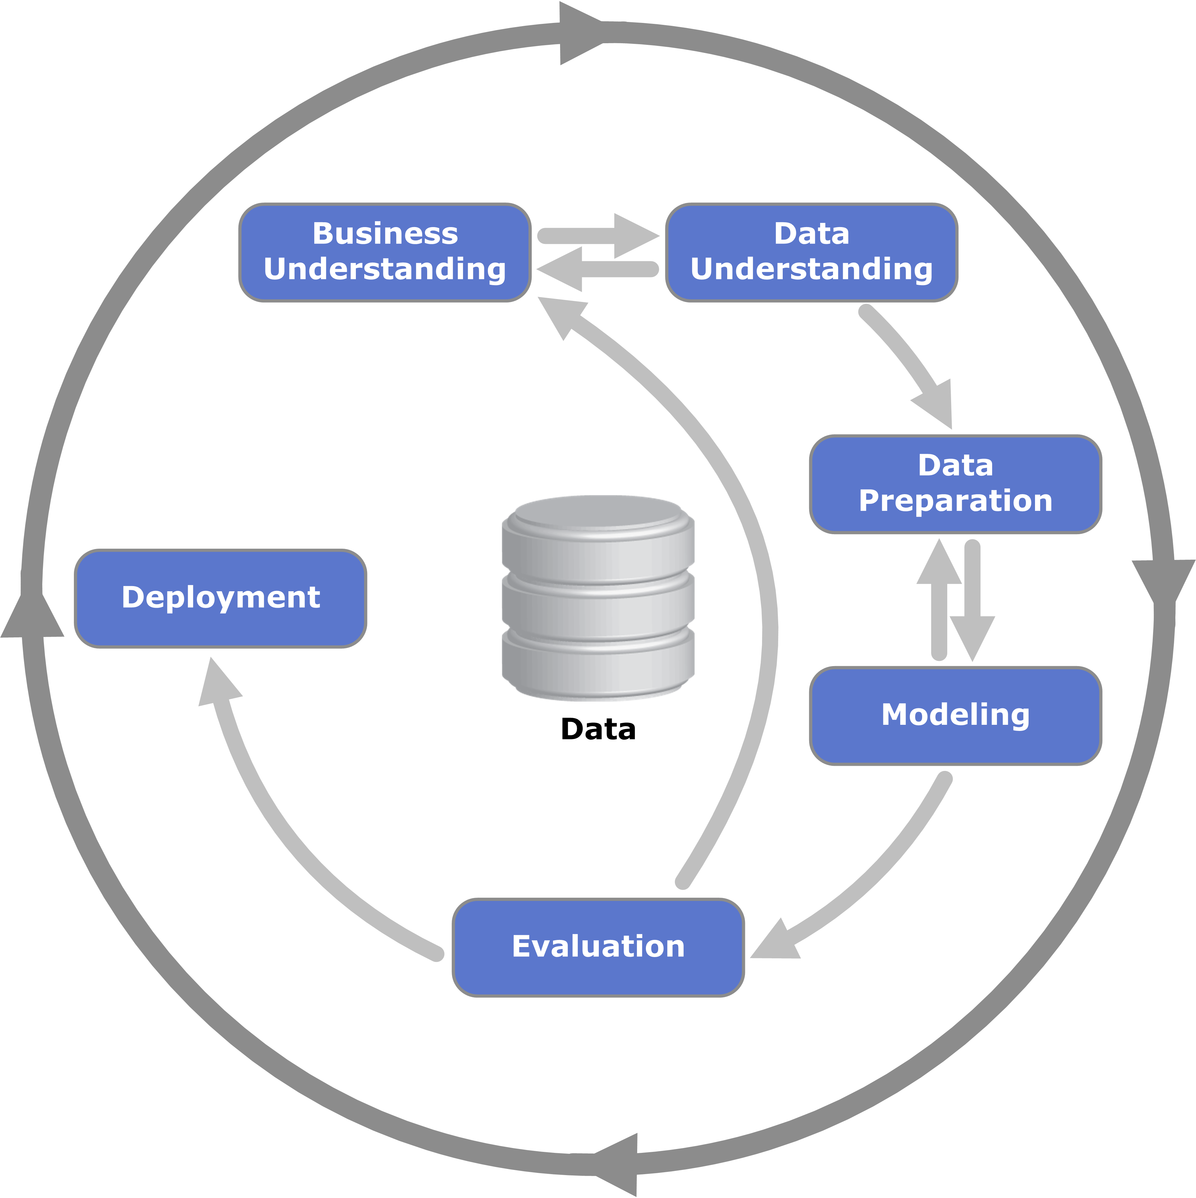
\includegraphics[width=1.0\textwidth]{figures/1196px-CRISP-DM_Process_Diagram.png}
    \caption{CRISP-DM 流程圖 (c)Kenneth Jensen, CC BY-SA 3.0} 
    \label{fig:CRISP-DM}
  \end{center}
\end{figure}

\begin{enumerate}
\item \textbf{定義領域問題}(Business Understanding):CRISP-DM~所定義的資料探勘步驟第一步要將希望解答的問題瞭解並定義清楚,有清楚明確的問題定義,才能夠規劃出需要收集哪些資料,用哪種類型的資料探勘方法來挖掘知識,解答問題。
\item \textbf{定義分析資料}(Data Understanding):有明確的問題定義之後,就能夠更深入的探討有哪些相關的資料,要解答此一問題所需要的相關資料為何,並且實際的去收集這些資料。
\item \textbf{資料前處理}(Data Preparation):此一步驟是資料探勘流程當中,相當重要的一個步驟,對於模型的品質優劣會有相當大的影響。會需要資料前處理的原因主要有兩個,第一個原因是由於現實世界的資料都會有很多雜訊在其中,像是人為輸入的錯誤、較為極端的離群案例資料等,因此在真正的訓練並建立模型之前,需要先把這些雜訊去除,這些雜訊在資料庫中的呈現通常為缺漏值、過大或過小的數值或是意義上不合常理的數值;另一個原因則是要將不同的輸入屬性的數值作整理,讓不同的資料探勘演算法可以更容易的根據不同屬性的特性來建立模型,這些前處理的方法包括了數值正規化、取指數對數、單位調整甚至是重新組合出新屬性,像是主成分分析法。
\item \textbf{建立模型}(Modeling):選擇適合該問題的資料探勘方法對前處理過的資料進行分析與模型建立,模型之建立工作包括了適合演算法的挑選以及不同演算法參數之挑選,兩者都是需要不斷嘗試並調整的工作。
\item \textbf{評估模型}(Evaluation):評估前兩步驟中所建立的模型品質是否符需求,並且要避免過適(overfitting)的現象,實務上是將資料分為訓練集與測試集兩組來驗證模型的可靠度,更為嚴謹的分析可以使用十群交叉驗證方法來處理,判斷的依據則根據不同的資料探勘方法有不同的模型品質指標,例如決定係數、線性關係、正確率等等。
\item \textbf{應用模型}(Deployment):將模型產出的知識實際納入應用,抑或是將探勘結果整理成完整的報告。
\end{enumerate}

其中資料探勘在收集完資料後的大部分的工作,均在資料前處理以及建立模型兩個步驟,此二步驟的操作對於最後產出模型之品質有相當大的影響。而本研究之流程較~CRISP-DM~之流程稍有不同,是先基於一個現有的特定領域的校舍耐震資料庫作分析,找出校舍耐震資料庫中各種潛藏知識的可能性,定義出這些知識所能夠解決的問題,詳細分析問題的需求,之後則是照著~CRISP-DM~的流程進行,從校舍耐震資料庫中挑選出相關的資料屬性,然後接著進行資料前處理、建立模型、評估模型幾個步驟。

資料探勘技術方法繁多,Fayyad~\cite{fayyad1996data}根據其處理的問題形式,將資料探勘的方法分為分類、分群、迴歸以及關聯等四種主要的問題類型。其中,分類方法處理的問題是用來判斷資料的類別,而且這些類別是已知的類別,例如將所有的校舍資料分類成有安全疑慮和沒有安全疑慮的方法就是屬於分類問題。分群問題和分類問題有點相似,一樣是將資料分成數個群組,最主要的差異是分群問題的各個群組的特性在一開始並不清楚,分群方法是將資料根據其屬性數值為依據,分析其相似度,把相似的放在同一個群組,不同群組的特性是要在分出群組後才能夠進行分析瞭解的。迴歸問題就是要用迴歸方法來從資料的屬性中,找出特定屬性與其他屬性間的關係模型,這些屬性間的關係可能是非線性的,而且沒有解析解的關係模型,因此常見的方法是用統計的方式,從現有的資料來反向歸納出關係方程式,又或著是用像類神經網路之類的機器學習方式,透過現有的資料來讓機器學習以求出關係模型,以校舍耐震資料庫來說,校舍耐震能力指標的預測就是一種迴歸問題,校舍耐震能力指標與其校舍的設計參數間的關係就是一個非線性關係,要得到兩者之間的非線性模型就需要用到回歸問題的分析方法,迴歸問題也是最常見的資料探勘問題種類。最後一種是尋找屬性間的關聯,這種問題的主要目標在尋找不同筆資料屬性間所存在的關係,舉例來說,使用校舍耐震資料庫的資料來作關聯分析,可能可以去尋找像是:五層樓的校舍的校舍長度深度有什麼趨勢,或是民國八十到九十年之間所建校舍的校舍走廊設計是否偏好有走廊柱等。本研究在定義好所欲解答的問題後,根據問題的性質判斷,使用的資料探勘方式以迴歸為主,分類分群的方法則是為輔助。

以下分別介紹本研究所使用到的各種分析方法,除建立模型的各種訓練和學習演算法外,還包括資料前處理和驗證所使用的分析方法以及驗證指標。


\section{資料前處理方法}

資料前處理方法常見的目的有:找出重要性較高的屬性、凸顯資料特性、剔除特異資料點等;本研究主要的資料過濾方法為資料的合理性分析,其是根據資料特性,根據經驗與專家意見等參考依據,建立出資料合理性的判斷方法。而除了合理性分析外,尚有較為簡單的數種方法,包括:

\begin{itemize}
\item 輸入屬性篩選
\item 子資料集挑選
\end{itemize}

輸入屬性篩選的主要目的在剔除和探勘目標不相關的資料屬性,減少資料維度,可以讓機器學習的效率更好;子資料集挑選是針對特定屬性,如果有非常不平均之分佈情形,例如一個二元指標,有很大比例的資料之值都相同,那就可以透過子資料集挑選的方法,將這一大類的資料挑出,和輸入屬性篩選一樣可以減少資料的複雜度。而除了以上的三種前處理方法外,還有主成分分析法,是透過數學統計分析求得最能夠代表資料變異的屬性。

\subsubsection{主成分分析}

主成分分析(Principal Component Analysis, PCA)是常見的前處理方法,它可以用來減少資料的維度,其數學原理是將資料向量投影到不同的座標系統,將原始的資料轉換成不同座標系的的向量資料,且能保持最大程度的,輸入屬性對於輸出屬性的貢獻,如圖~\ref{fig:pca}\cite{ben2013pca}~所示,在一個~X~Y~座標系統中分佈的資料點,可以透過~PCA~分析,找到兩個更能夠代表資料特性的屬性座標軸~$\sigma^2_{signal}$~和~$\sigma^2_{noise}$。

\begin{figure}[hbtp]
  \begin{center}
    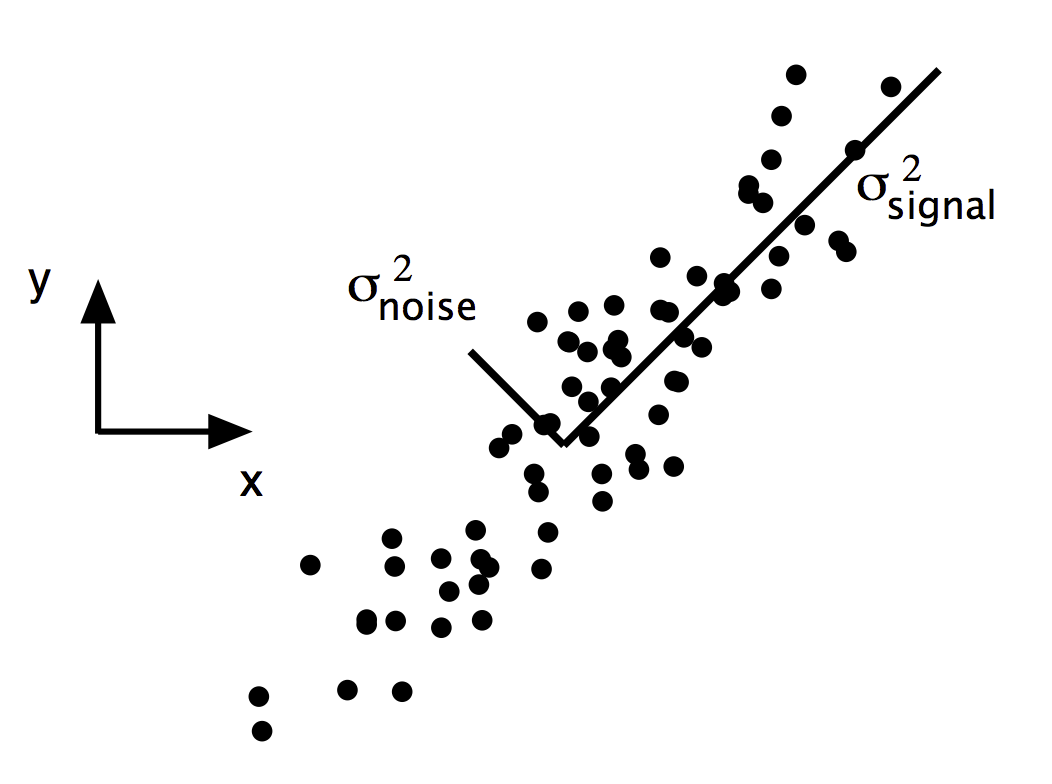
\includegraphics[width=0.6\textwidth]{figures/pca.png}
    \caption{主成分分析原理} 
    \label{fig:pca}
  \end{center}
\end{figure}


% PCA, a very common data preparation method, can identify very important attributes among various attributes. The goal is to convert the original variables through vector transition into mutually independent variables of a linear combination. The ideal situation is that principal components obtained from linear combination retain most of the information of original variables.

\section{資料探勘方法}

資料探勘的方法分為分類、分群、迴歸以及尋找關聯~\cite{fayyad1996data}~,其中迴歸是最常使用到的一種,本研究的主要目標皆可以歸納為迴歸類的問題,因此使用到的迴歸演算法最多,接著才是作為輔助用的分類和分群演算法。

迴歸、分類、分群三種資料探勘所建立的模型可以簡單的定義為:

\begin{equation} y = f(x) \label{eq:ModelEqu}\end{equation} 

$f(x)$~就是透過資料探勘分析學習而得到的模型函數,~$x$~代表輸入參數,輸入參數是各種已知的屬性資料,例如可以簡單透過量測得到的校舍尺寸資訊,~$y$~則是代表輸出參數,也就是希望透過這個模型所得到的,比較難取得的屬性資料,例如需要經過詳細評估才能的到的校舍~$CDR$~值、或是校舍分類的類別索引。

\subsection{迴歸方法}

\subsubsection{Generalized Linear Model}

廣義線性模型是由Nelder and Wedderburn~\cite{citeulike:5485398}所提出,比起迴歸分析(simple regression)更為彈性,此模型是假設資料點的分佈有一分佈模式,且輸入參數~$x$~與輸出參數~$y$~之間的關係是由一連結函數(Link Function)建立,如~log function、power function~等,其定義之~$x$~與~$y$~間之關係模型如下:


\begin{equation} g(E(y)) = x\beta + O, y \sim F \label{eq:GLM}\end{equation} 

$g(.)$是為所選的鏈結函數,$E(y)$~是~$y$~的期望值,~$O$~是偏移(offset)變數,~$F$~則是~$y$~的分佈模型,其是用牛頓法(Newton-Raphson Method)不斷的調整~$\beta$~使的~$x\beta + O$~逼近~$g(E(y))$~,最後最接近的方程式即為~$x$~與~$y$~兩者的關系式。比起迴歸分析,此方法還需要了解~$y$~值分佈狀況,選擇出最適合的分佈函數,並假設~$x$~與~$y$~間的鏈結函數形式,雖然越多的參數選擇代表了更多的模型不確定性,但廣義線性模型卻能夠提供比迴歸分析更廣的應用範圍,也可能得到更接近真實的關係模型。


\subsubsection{類神經網路}

類神經網路(Artificial Neural Networks,ANNs),其是希望能模擬建構出人腦內的神經網路,以處理各種複雜的問題,人類大腦是由大約千兆個神經元(Neuron)所構成,而每個神經元又會和其他約一萬個神經元連結,構成一個龐大且複雜的神經網路,這樣複雜的一個神經網路讓人類可以學習並了解各種事物與知識。McCulloch and Pitts~\cite{mcculloch1943logical}所提出的模型為後續類神經網路發展的雛形,而目前最為被廣泛使用的類神經網路結構為倒傳遞類神經網路(Back-Propagation Network, BPN),為一種監督式學習網路,應用十分廣泛。Werbo~\cite{werbos1974beyond}首先提出隱藏層及倒傳遞學習理論的概念,但在當時並未受到重視。直到~Rumelhart~及~McClelland\cite{rummelhart1986learning}於~1986~提出~BPN~學習演算法及通用差距學習法則(Generalized Delta Learning Rule),採引起學者的廣泛討論。倒傳遞演算法是將一組樣本~1/0~問題變為一個非線性最佳化的問題,其基本原理是利用最陡梯度下降法(Gradient Steepest Descent Method)以計算且調整網路權重,使推論輸出值與目標輸出值間的誤差最小化,得到精確的學習。因此,倒傳遞類神經網路是用於診斷與預測上,若將此模式視為輸入與輸出間的映射關係,則~BPN~演算法是一種輸入輸出的映射過程,一個標準的~BPN~類神經網路可以分為輸入層(input layer)、隱藏層(hidden layer)、輸出層(output layer),其結構如圖~\ref{fig:ANN-network}\cite{larose2005discovering},分別介紹三種神經元如下:

\begin{description}
  \item [輸入層神經元]
  用以表現網路的輸入變數,其處理單元數目依問題而定,通常相等於所使用的輸入參數,使用線性轉換函數,即~$f(x)=x$。
  \item [隱藏層神經元]
  用以表現輸入處理單元間的交互影響,其處理單元數目並無標準方法可決定,經常需以試驗方式決定其最佳數目,使用非線性轉換函數,網路可以不只一層隱藏層,也可以沒有隱藏層。
  \item [輸出層神經元]
  用以表現網路的輸出變數,其處理單元數目依問題而定,使用非線性轉換函數。
\end{description}

\begin{figure}[hbtp]
  \begin{center}
    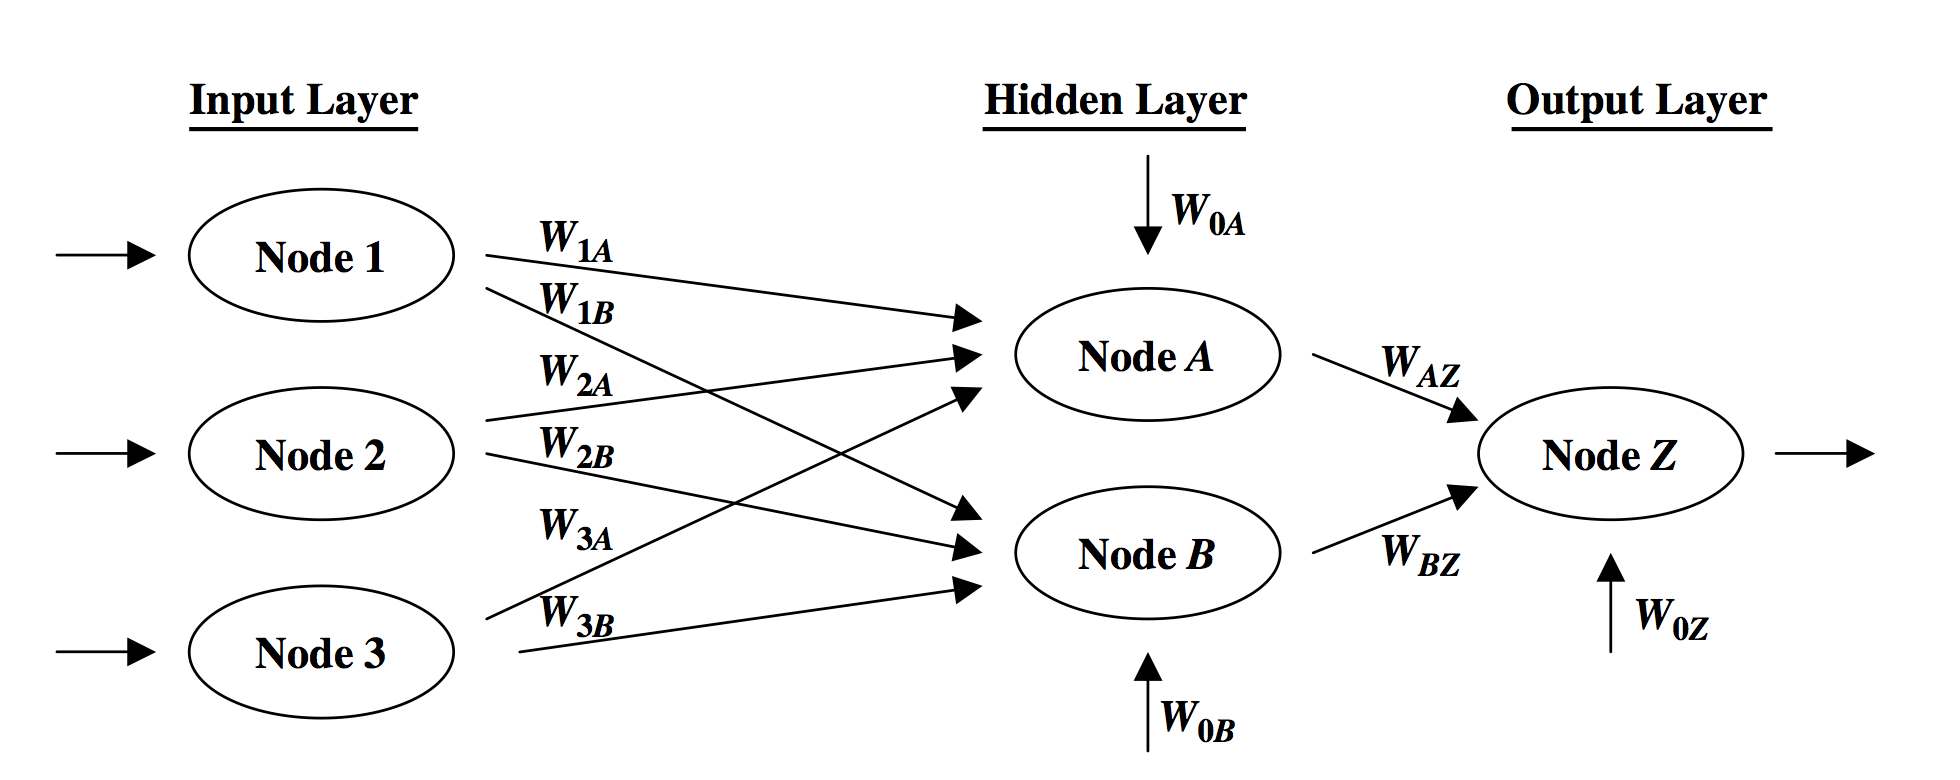
\includegraphics[width=1.0\textwidth]{figures/anns-network.png}
    \caption{類神經網路結構圖} 
    \label{fig:ANN-network}
  \end{center}
\end{figure}

處理單元其輸出值及輸入值的關係式,一般可用輸入值的加權乘積和之函數來表示:

\begin{equation}\begin{split}  Y_j &= f(net_j) \\ net_j &= \sum W_{ij}X_i - \theta_j \label{eq:anns}\end{split}\end{equation} 

其中,$Y_j$~為輸出層第~$j$~個處理單元之推論輸出值,$net_j$~為輸出層第~$j$~個處理單元之集成函數,$W_{ij}$~為第~$i$~個輸入層單元與第~$j$~個輸出層單元間之連結權重。$X_i$~為輸入層第~$i$~個處理單元之輸入值。$\theta_j$~為輸出層第~$j$~個處理單元之閥值,$f$~為轉換函數,是為神經元從輸入層加總轉換至輸出的一種映射規則亦是將非線性的影響導入網路中的一種設計。而轉換函數的選擇相當多, 本研究採用的轉換函數為對數雙彎曲函數,如下所示:

\begin{equation} f(x) = \dfrac{1}{1 + e^x}  \label{eq:annsf}\end{equation} 


\subsubsection{基因規劃}

基因規劃(Genetic Programming,GP)是基於基因演算法(Genetic Algorithm, GA)發展而來,而~GA~是~1975~年由~John Holland\cite{holland1975adaptation}~所提出的演化求解方法,其是基於生物演化的過程為基礎,假設問題的目標可以轉換為二元的基因序列,再透過模擬生物交配、突變的進化過程,求得最佳化問題的解,和傳統的演化求解方法相比,基因演算法可以比較容易的找到全域最佳解,且其可以快速的找到足夠好的解,即使問題的複雜度很高。基因演算法的應用領域相當廣泛,在營建領域也有不少的應用,Huang...et. al.\cite{minshui2009study}~就使用GA預測梁模型受力後會產生破壞的位置及其嚴重性,Šešok和Belevicius\cite{vsevsok2008global}~則使用基因演算法建立一個~truss topology~最佳化的建議系統。

基因規劃則是~1992~年由~Koza\cite{koza1992genetic}~所發表的方法,它是基於發展許久的基因演算法而來,將基因演算法所要演進發展的基因序列換為樹狀結構的分析樹(parse tree),並藉由與基因演算法相同概念的交配、突變和篩選等機制來達成解析樹的演化,並達成最佳化目標,如果要求得一數學關係方程式,則可以使用運算樹(operation tree)作為欲演進的解析樹結構。運算樹是一個二元樹結構,如圖~\ref{fig:GP-struct}~,其底層的末端點是方程樹的輸入變數或是其它常數、數值等,其餘的分支節點都是運算子(operator),藉由置換各個節點的輸入數值和運算子,就可以組成各種可能的數學方程式。此一方法的特色是其模型之輸出形式即為輸入~$x$~和輸出~$y$~的關係方程式,且其方程式之形式不受限於基因演算法之特性。在營建領域使用~GP~加上運算樹進行最佳化的應用少有人做,Yeh and Lien\cite{yeh2009knowledge}~使用GP方法來預測混凝土強度。Tsai\cite{tsai2011using}~則使用修改過的~Weighted Genetic Programming~方法建立出~squat wall strengths~的方程式,並且還利用一些修剪公式的方法來調整得到的公式,讓公式可以更精簡,但是還保留有一定程度的可靠度。

\begin{figure}[hbtp]
  \begin{center}
    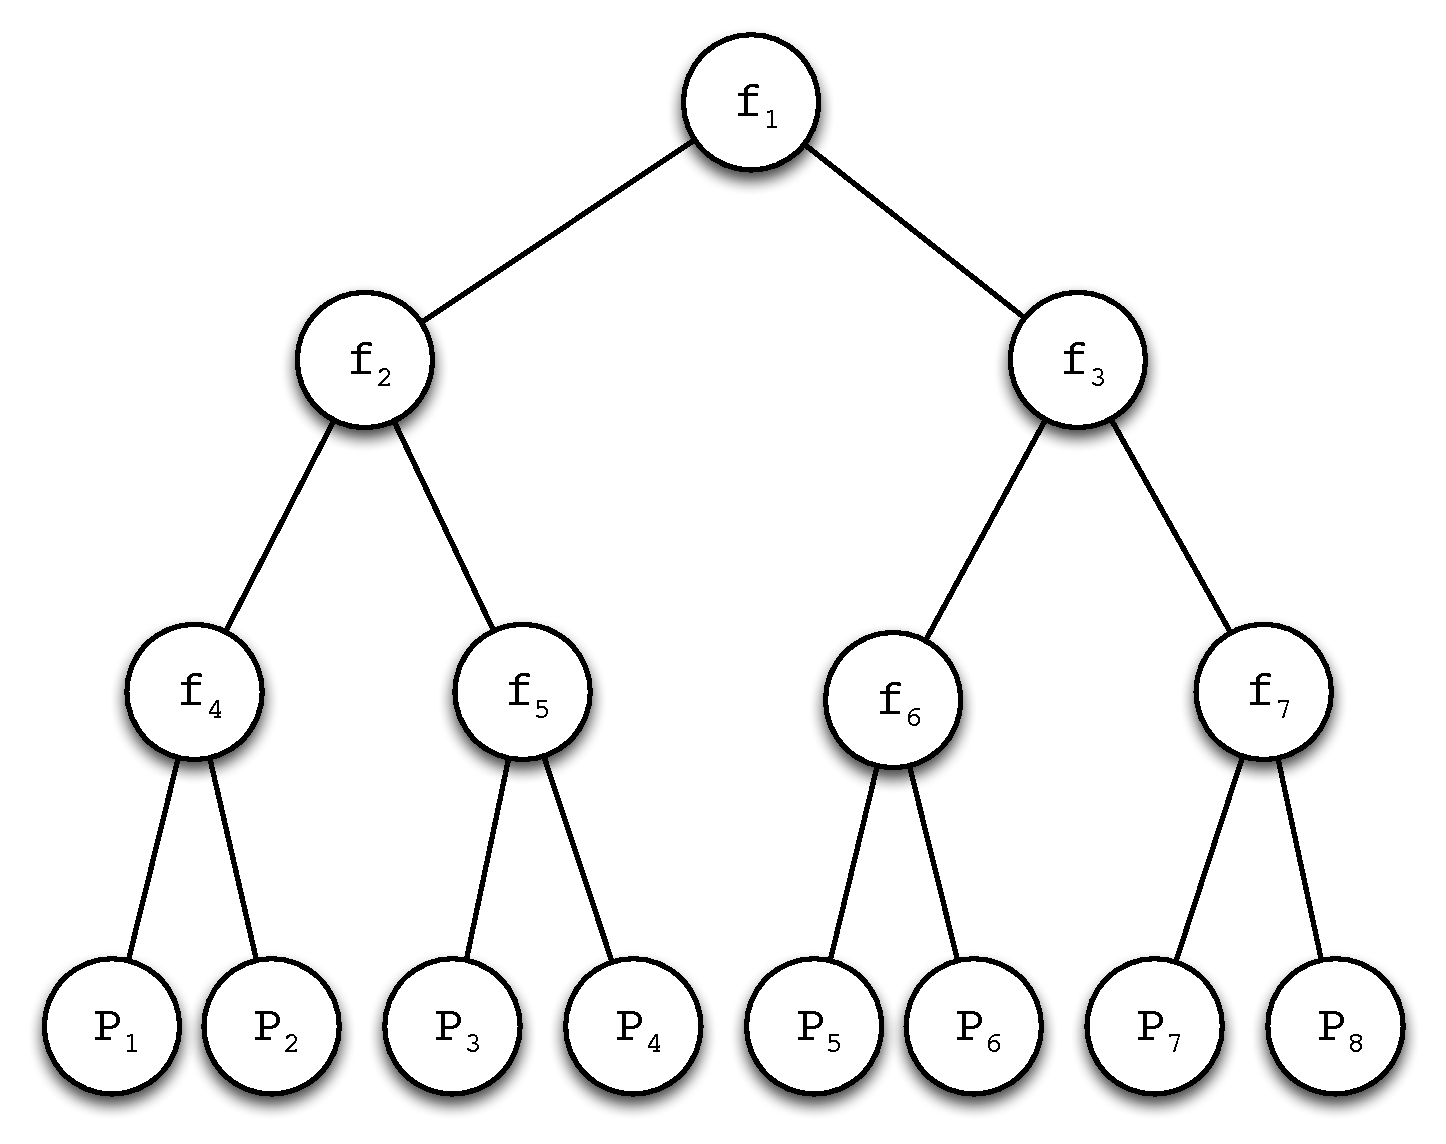
\includegraphics[width=1.0\textwidth]{figures/gp-struct.pdf}
    \caption{GP 運算樹結構示意圖} 
    \label{fig:GP-struct}
  \end{center}
\end{figure}

基因規劃藉由這樣的運算樹設計,再透過基因演算法最佳化輸入參數的選擇、不同運算節點的運算子,便可以根據資料建立出一個屬性與所求目標的關係方程式。

\subsubsection{加權基因規劃}

加權基因規劃(Weighted Genetic Programming,WGP)是由~Tsai\cite{tsai2011predicting}~所提出,基於~GP~ 方法發展而來,不同之處在於其運算樹的每個節點前都加上一個權重~$w$~,最佳化的過程除了對方程式結構和參數的選擇最佳化外,還要同時最佳化所有的權重,因此其輸出的關係方程式可能性遠大於~GP~方法,故可以處理更為複雜的問題。~WGP~的運算樹結構如圖~\ref{fig:WGP-sample}~,每個運算樹都可以組成一個數學方程式,如圖~\ref{fig:WGP-sample}~之運算樹即可組成方程式如下:

\begin{equation} w_1(w_3(\dfrac{w_7P_2}{w_8P_6}) - w_4sin(w_9\bar{C}))+w_2 \times cos(w_{12}c \times w_{11}P_1) \label{eq:WGP-sample}\end{equation} 


\begin{figure}[hbtp]
  \begin{center}
    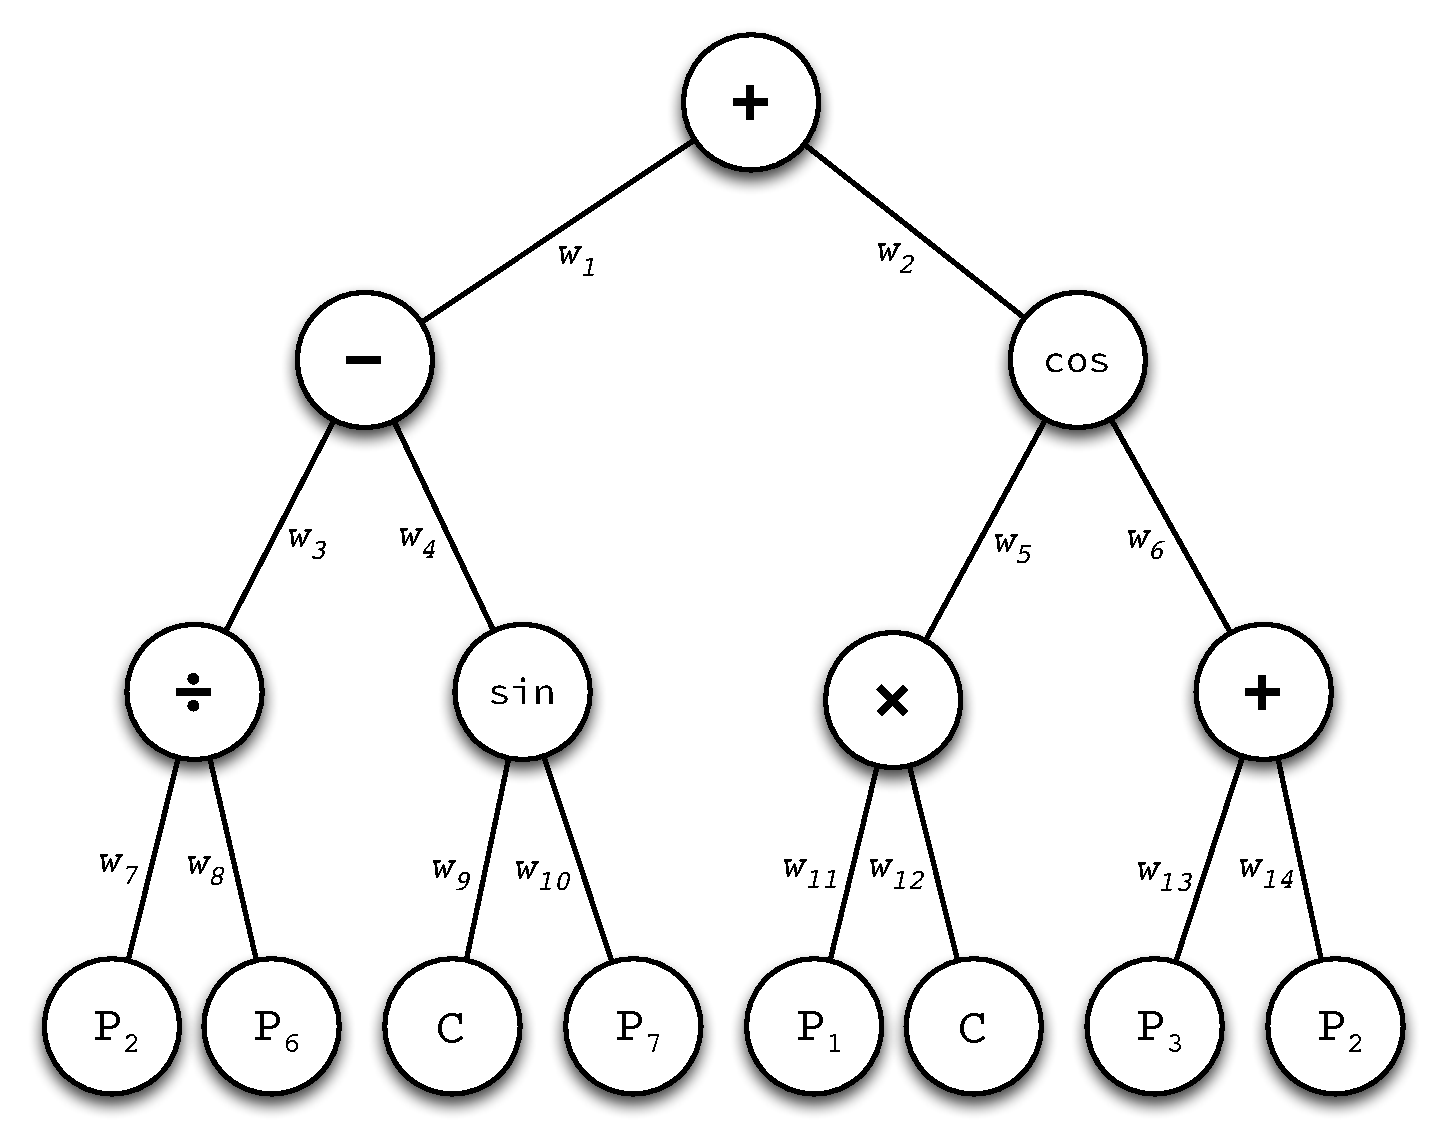
\includegraphics[width=1.0\textwidth]{figures/wgp-sample.pdf}
    \caption{WGP 運算樹結構示意圖} 
    \label{fig:WGP-sample}
  \end{center}
\end{figure}


運算樹可以分為兩種層級,運算層全部都是運算子節點,輸入層則是輸入參數的選擇,運算層每多一層,需要最佳化的節點和權重都會以等比級數成長,運算層的層數也影響到最佳化結果的方程式複雜度,而輸入層則全部都是輸入節點,每層之間的每個連結都有一個權重參數,這些權重即為~WGP~方法最大的特色,這些權重可以讓運算樹組成的方程式有無限多種,也可以用以表示不同參數的重要性,因此雖然加入權重會讓最佳化更費時間,但仍然值得加上權重。

圖~\ref{fig:wgp-unit}~是一個構成~WGP~運算樹的基本單元,和圖~\ref{fig:gp-unit}~所示的~GP~運算樹的基本單元類似,包含一個父層節點和兩個子層節點,父層的節點是運算節點~$F$,透過權重參數連接到兩個子層節點,子層節點可能是其它的基本單元或是輸入節點,而整個基本單元的輸出~$y$~為:

\begin{figure}
  \begin{center}
    \subfigure[GP]{
      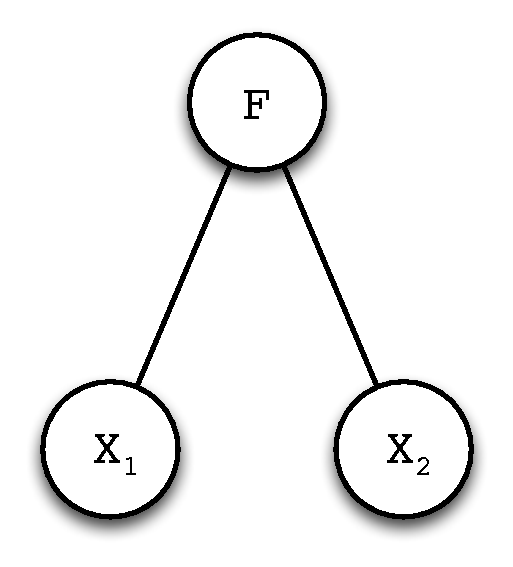
\includegraphics[width=0.4\textwidth]{figures/gp-unit.pdf}
      \label{fig:gp-unit}
    }
    ~
    \subfigure[WGP]{
      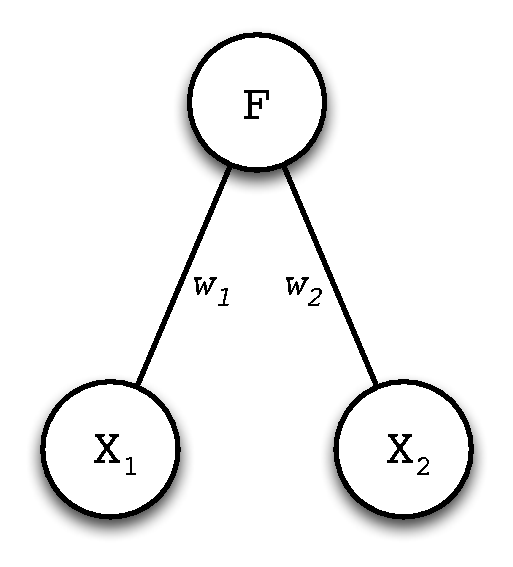
\includegraphics[width=0.4\textwidth]{figures/wgp-unit.pdf}
      \label{fig:wgp-unit}
    }
    \caption{GP 系統之單位元素}
    \label{fig:gps-units}
  \end{center}
\end{figure}

\begin{equation} y = \text{one of}\;\begin{cases}
  f_1 = w_1x_1 + w_2x_2 \\
  f_2 = w_1x_1 - w_2x_2 \\
  f_3 = w_1x_1 \times w_2x_2 \\
  f_4 = w_1x_1 \div w_2x_2 \\
  f_5 = \abs{w_1x_1}^{w_2x_2} \\
  \hphantom{f_1\;\;}\vdots \\
  f_n = \dfrac{1}{sin(w_1x_1)+cos(w_2x_2)}
\end{cases} \label{eq:WGP-y}\end{equation}

運算子~$F$~可能有數種選擇,同時配合最佳化演進得來的權重和子層節點的~$x_1$、$x_2$~,便可以計算得到這個基本單元的輸出~$y$,而子層節點的~$x_1$~和~$x_2$~有兩種可能的來源,一是此一基本單元的子層仍為運算層,則其數值要藉由計算該基本單元而來,另一種可能是子層為末端的輸入層,則~$x_1$~、~$x_2$~的值如下:

\begin{equation} x_i = \text{one of}\; \{1, P_1, P_2, P_3, \cdots P_j, \cdots P_{NI}\},\; j = 1 \sim NI \label{eq:WGP-xi}\end{equation}

其中~$NI$~為輸入參數的數量,$P_j$~為第~$j$~個輸入參數,$x_1$、$x_2$可能為輸入參數的任一個,而輸入參數也可能為常數~$1$。

運算樹的層數~$NL$~定義為有運算節點的層數,即運算層的層數,運算樹的層數大小會影響到需要最佳化的基因數量~$N_g$,其公式為:

\begin{equation} N_g = 2^{NL} - 1 + 2^{NL} + 2^{NL + 1} - 2 = 2^{NL + 2} - 3  \label{eq:WGP-N}\end{equation}


其中運算層節點的函數選擇有~$2^{NL} - 1$~個、參數層的參數選擇有~$2^{NL}$~個、以及參數的權重~$w$~有~$2^{NL + 1} - 2$~個。藉由這樣的運算樹設計,再透過~GA~最佳化輸入參數的選擇、不同運算節點的運算子和各個節點不同的權重,~WGP~方法便可以根據資料建立出一個屬性與所求目標的關係方程式。


\subsubsection{CHAID 決策樹}

CHAID(Chi-squared Automatic Interaction Detector)是由~Kass\cite{kass1980exploratory}~在~1980~所正式定名的建立決策樹的演算法,圖~\ref{fig:Decision-Tree-sample}\cite{kass1980exploratory}~即為一個典型的決策樹,決策樹是一個從根節點開始,然後根據數入屬性得資料以及不同分支的條件,移動到不同子節點,最後到達的節點的目標值即為此筆輸入屬性的預測值。CHAID~是利用卡方檢定來分析判斷輸入屬性的分割合併點,並根據不同輸入屬性對目標屬性的顯著性($p$-value)來挑選不同節點分割所依據的輸入屬性,依此建立出決策樹的分割點,可以建構出兩個以上分支的決策樹,有別於只有兩個分支的二元樹。決策樹一般是用來做分類形式的資料探勘,無法處理數值形式的迴歸,不過如果先將目標屬性區段化,則決策樹方法也可以建立出迴歸形式、用以預測數值的迴歸樹,不過由於其模型之性質,預測之目標屬性數值會分佈在特定數個數值。

\begin{figure}[hbtp]
  \begin{center}
    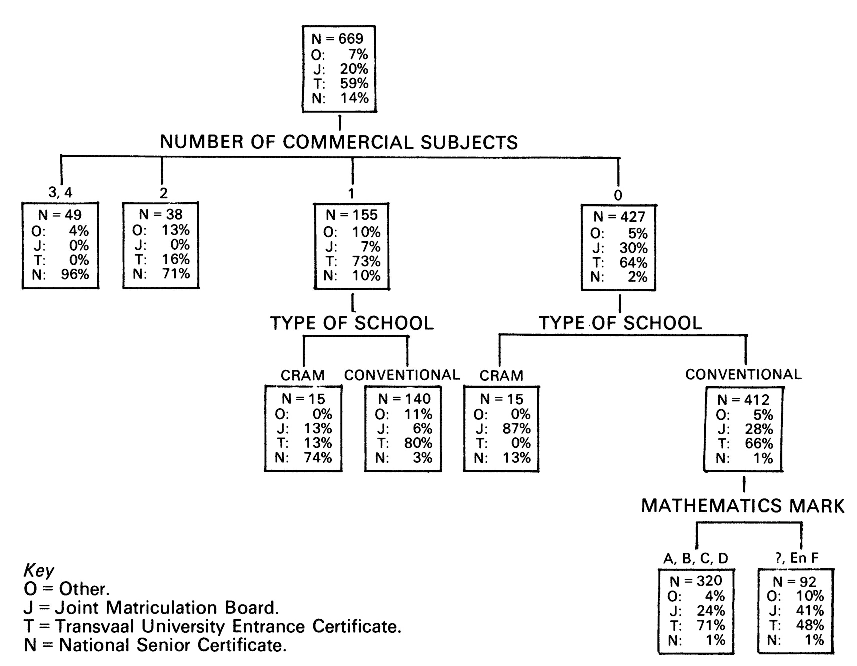
\includegraphics[width=0.8\textwidth]{figures/decision-tree.pdf}
    \caption{決策樹示意圖} 
    \label{fig:Decision-Tree-sample}
  \end{center}
\end{figure}


\subsection{分類方法}

\subsubsection{支持向量機}

支持向量機(Support Vector Machine, SVM)最早是BOSER~\cite{boser1992}等人,在~1992~年的~COLT(Computational Learning Theory)所提出,~SVM~是一個基於統計學習理論的分類方法,用來處理二元分割的問題,其原理是將原本無法線性分割的問題如圖~\ref{fig:svm}(a)\cite{verplancke2008support},將資料點轉換到一個不同維度的空間(kernel)後,假設該空間存在一超平面(hyperplane)如圖~\ref{fig:svm}(b),此一超平面可以正確的將資料分開,並將尋找此一超平面的問題轉換為一最佳化問題,求解後將此一超平面轉換回原本維度的空間即可得到二元分割邊界的方程式。而除了分類問題,Harris Drucker, et. al.,\cite{drucker1997support}~將此二元分割問題轉換為迴歸分析問題,故~SVM~也可以處理迴歸問題。

\begin{figure}[hbtp]
  \begin{center}
    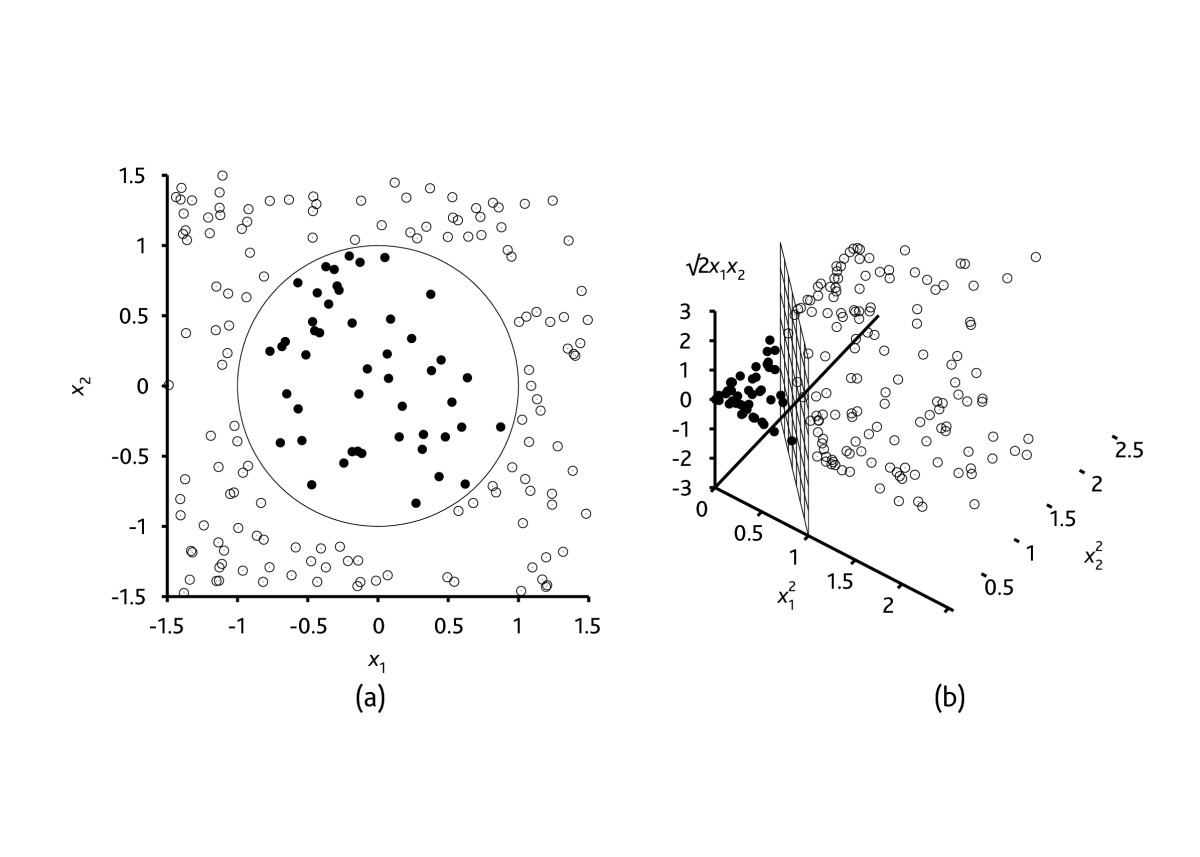
\includegraphics[width=1.0\textwidth]{figures/svm.jpg}
    \caption{SVM 示意圖}
    \label{fig:svm}
  \end{center}
\end{figure}

\subsection{分群方法}

\subsubsection{K-means}

K-means~是由~MacQueen\cite{macqueen67}~所提出,也是最常被使用的分群演算法之一,屬於機器學習方法,其主要步驟為:

\begin{enumerate}
\item 使用者決定要將資料分為幾個群集,群集數為~$K$~。
\item 將資料隨機分到~$K$~個群組,並且計算出此時分群狀態下的每個群組的中心點。
\item 將每個資料點重新分群到新的群組,新群組的選擇方法為中心離它最近的那個群組。
\item 用新的分群狀態計算出新的群組中心點。
\item 重複步驟~3~和~4~直到每個資料點的群組都穩定不再變化。
\end{enumerate}


% As proposed by MacQueen~\cite{macqueen67}, K-means is one of the most common clustering methods and has a wide application scope. Notably, it is a machine learning method; its principal steps are as follows.


\subsubsection{兩步分群}

由於各種學術、商業研究所處理的問題資料量越來越大,分群演算法所需要的運算時間也急遽的成長,為了讓分群演算在處理大量的資料時也能有良好的效能表現,而發展出兩步分群法(Two-Step Clustering),其是由~Zhang~、~Ramakrishnan~與~Livny\cite{zhang1996birch}~所提出,此一方法分為兩個主要步驟:第一步是先把資料依據其與相鄰資料的相似度來排序並分成數個小群集,相似度的計算則是使用~log-likehood~函數,接著第二步再使用階層式分群方法,將這些群集慢慢組合或拆分直到達成停止條件。其特色在於運算複雜度較其他演算法來的低,例如~K-means~演算法就需要不斷的重複運算直到所有的資料歸屬都收斂不再變化為止,因此資料量成長時也不會讓運算時間成長到無法應用的程度。

% Based on of the massive volume of basic data for school buildings in the database, this study chooses two-step clustering method. The basic concept was first proposed by Zhang, Ramakrishnan and Livny~\cite{zhang1996birch} for handling large amounts of data. This method has two major steps. The first step sequences data and pre-clusters sequences into small subclusters based on the similarity of adjacent data, thereby reducing the amount of data. The second step divides several small subclusters into the desired number of clusters using a hierarchical clustering method. The hierarchical clustering method then combines close subclusters slowly until the stop condition is met. The computing speed of this method is influenced slightly by the volume of data.

%\section{探勘結果驗證方法與指標}
\section{探勘結果指標}

%\subsection{驗證方法}

%\subsubsection{10 fold cross validation}

%\subsection{結果指標}

要驗證資料探勘所取得模型的可靠度如何,有很多的指標可以使用,分別可以從不同的角度呈現出模型的優劣,而本研究使用決定係數~$R^2$~做為判斷模型優劣的主要指標,並以其他的指標來做為輔助。

\subsubsection{敏感度分析}

敏感度分析並非用來判斷模型的優劣之用,而是用來判斷不同的輸入屬性,其資料的變異與輸出目標資料變異間的關係,定義為:

\begin{equation}  S_i = \dfrac{V(E(Y|X_i))}{V(Y)} \label{eq:sensitivy}\end{equation} 

其中~$S_i$~是第~$i$~個輸入參數的~Sensitivity Index,$V(Y)$~是目標屬性的變異數,而~$E(Y|X_i)$~是目標屬性隨著第~$i$~個輸入參數變化的期望值,$V(E(Y|X_i))$~則是此一數值之變異數,$S_i$~的值介於~0~到~1~之間,數值越高表示輸出目標對此一輸入屬性的敏感度越高,可以認為是重要度較高的輸入屬性。


\subsubsection{決定係數}

決定係數(coefficient of determination)又稱為~$R^2$~,其公式為:

\begin{equation} R^2 = 1 - \dfrac{SS_{res}}{SS_{tot}} = \dfrac{SS_{reg}}{SS_{tot}} = \dfrac{\sum{(\hat{y_i} - \tilde{y})^2}}{\sum{(y_i - \tilde{y})^2}} \label{eq:RSQ}\end{equation} 

其中 $y_i$ 是關係模型輸出屬性之值, $\hat{y_i}$ 則是該輸出屬性之實際值,$\tilde{y}$ 則是所有資料的輸出屬性實際值之平均,透過此一指標可以了解輸出屬性中有多少比例的資訊是由輸入屬性的變量所產生的,也代表著關係模型的正確性,而其值恰巧為關係係數\cite{aldrich1995correlations}~$R$(correlation coefficient)的平方,透過關係係數可以了解實際的輸出屬性數值與透過關係模型得到的推估值之間的線性關係,其值之範圍為~$0 \sim 1$,線性關係越高表示兩者之間越接近,也代表著關係模型所建立關係之正確性。

\subsubsection{平均絕對百分比誤差}

平均絕對百分比誤差(Mean Absolute Percetage Error, MAPE)~的公式如下:

\begin{equation} \text{MAPE} = \dfrac{\sum{\dfrac{\abs{y_i - \hat{y_i}}}{\hat{y_i}}}}{N} \times 100\% \label{eq:MAPE}\end{equation}

其中~$N$~是資料的總數,~$y_i$~是使用探勘得到的關係模型所求得的輸出屬性預測值,~$\hat{y_i}$~則是該屬性的實際值,此一指標代表了模型產出結果的平均誤差,可以呈現模型的準確度,數值越低代表模型品質越好。


\subsubsection{均方根誤差}

均方根誤差(Root Mean Squared Error, RMSE)定義如下:

\begin{equation} \text{RMSE} = \sqrt{\dfrac{\sum{(y_i - \hat{y_i})^2}}{N}} \label{eq:RMSE}\end{equation}

其中~$N$~是資料的總數,~$y$~是透過資料所建立的關係模型所求得的輸出屬性預測值,~$\hat{y}$~則是輸出屬性的實際值,此一指標代表了模型產出結果的平均誤差,數值越低越好,和~MAPE~相比,其差異在~MAPE~只表現了模型輸出數值的誤差平均,而~RMSE~還包含了誤差量的離散度資訊在內,~MAPE~表現相同的模型,其單筆資料誤差值分布越離散,~RMSE~的表現會越差,其可接受範圍則要根據輸出屬性的數量級和問題複雜度而定。


\subsubsection{命中率}

命中率(hit rate)是用來判斷關係模型的正確率的,判斷連續數值形式的模型正確率時,其定義為:

\begin{equation} \text{Hit Rate} = \dfrac{ \sum{I\{(1 - \alpha)y_i \le \hat{y_i} \le(1 + \alpha)y_i \}} }{N} \label{eq:hitratenum}\end{equation} 

其中~$I\{L\} \in \{0, 1\}$~,如果~$L$~為真,則~$I\{L\}$~為~1~,反之則為~0~,~$y$~是透過資料所建立的關係模型所求得的輸出屬性預測值,~$\hat{y}$~則是輸出屬性的實際值,而~$\alpha$~為命中率的容許誤差,且~$0 \le \alpha \le 1$~,如果~$\alpha = 0.1$~則表示誤差~$10\%$~內都算是有預測模型有預測命中,如果是判斷非連續數值形式的目標正確率時,例如布林值,其定義為:

\begin{equation} \text{Hit Rate} = \dfrac{ \sum{I\{y_i = \hat{y_i}\}} }{N} \label{eq:hitrate}\end{equation} 

此公式表示關係模型之目標為非連續數值形式時,要完全預測正確才會記入命中,命中率越高代表關係模型的結果越好,是一個非常直觀的模型品質指標。



\section{探勘目標分析}

由於本研究之目標在於使用各種不同形式之資料探勘方法,盡量的發掘校舍耐震資料庫中的隱含知識,因此研究的第一個步驟便是根據資料探勘方法的特性,以及校舍耐震資料庫當中所及的各種校舍資料,分析各種可能得到的知識,而根據四種主要的資料探勘知識形式及校舍耐震資料庫,分析可能可以從中探勘得到之知識如圖~\ref{fig:bigpicture}~所示。

\begin{figure}[hbtp]
  \begin{center}
    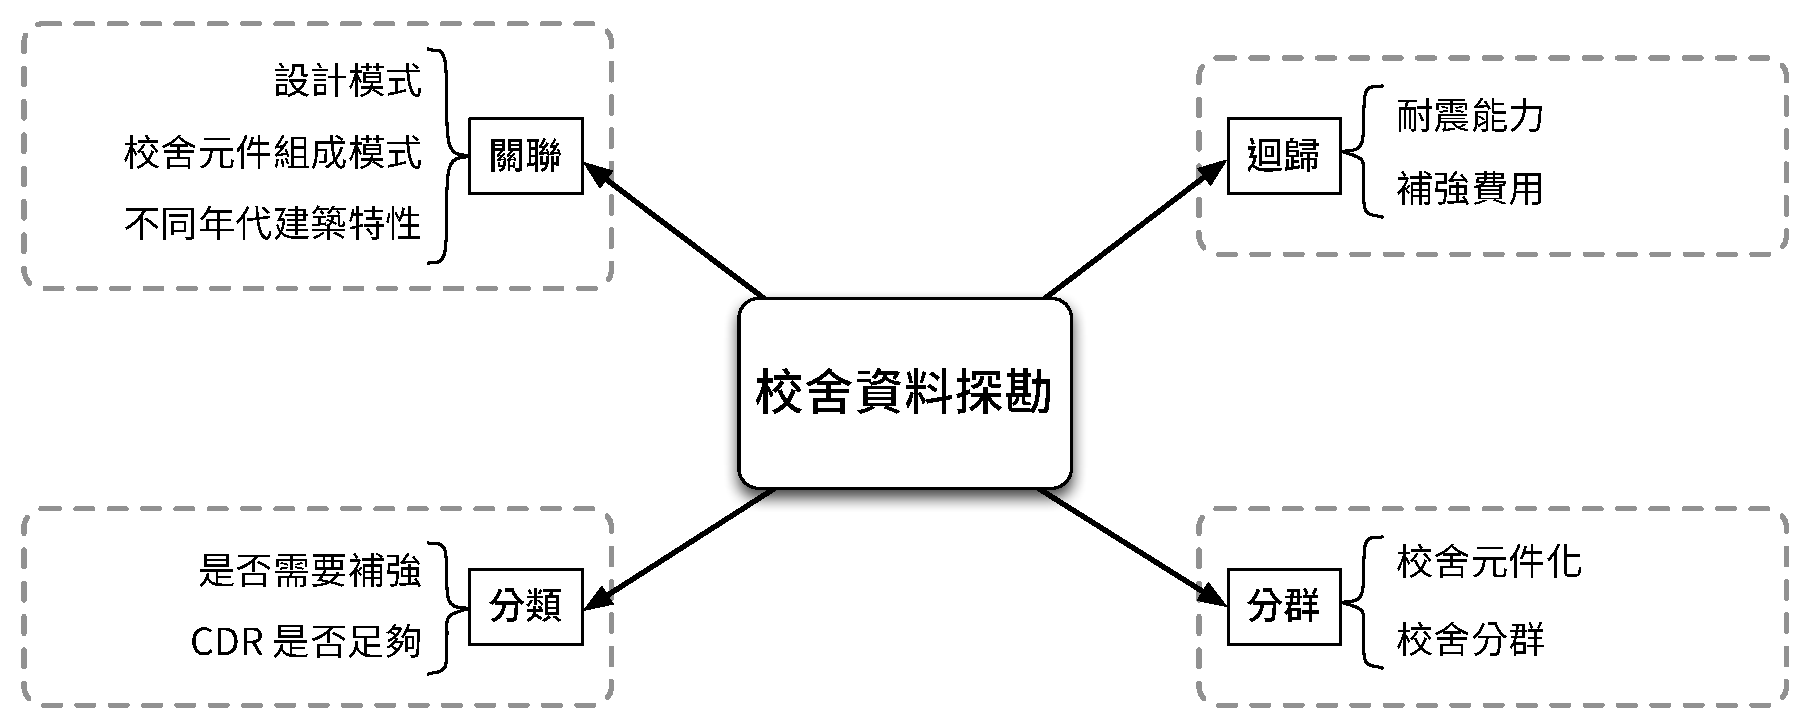
\includegraphics[width=1.0\textwidth]{figures/big-picture.pdf}
    \caption{知識挖掘規劃} 
    \label{fig:bigpicture}
  \end{center}
\end{figure}

其中,迴歸是屬於最常見的資料探勘形式,本研究所設計之迴歸形式的探勘問題包括了初步評估的~$Is$~值、詳細評估的~$CDR$~值、補強實際所花的總工程費等,在校舍耐震補強計畫中,不同階段的階段目標數值的迴歸關係模型,這些數值都是屬於連續性的數值,其數值應該與調查所得的校舍特性之間有所關聯;分類形式的知識則是以校舍是否需要補強這個詳細評估後得到的二元指標做為探勘的目標,校舍是否需要補強是整個耐震能力補強計畫當中一個非常重要的資料,如果可以透過關係模型來得知校舍是否需要補強,應該能夠讓校舍耐震能力補強計畫前半的篩選工作更有效率的執行,而在實際進行資料探勘研究後,還設計了另外一個知識探勘目標,詳細評估後的構件破壞情形與其設計參數、現況間之關係,校舍受到地震力後的構件破壞資訊可以讓,;分群形式的知識則設計有兩個,第一個是基本的校舍分群,將相近的校舍歸在同樣的群集當中,一來可以分析群集是否有顯著的特性可以探討,二來群集的資訊也可以做為其它資料探勘的參考輸入資訊。第二個分群的探勘目標是希望能夠將台灣典型校舍的結構,拆分成一些基礎的組成元件,例如教室、走廊、樓梯間等等,然後將不同的元件的各種可能模型,透過分群的方式找出,可能可以找到~10~種教室的形式、6~種走廊的配置等等,然後就可以將這些元件組合出台灣各種典型校舍,並且根據所挑選的元件,就可以得到一個可靠度足夠的校舍結構模型,並可以用來做一些模擬分析;最後則是關聯形式的知識,這類型的知識主要是可以呈現出不同的資料屬性間的趨勢與關係,因此設計上希望可以得到的知識包括了從校舍設計參數間找出校舍的主要模式,不同年代的校舍設計特色等。

而在這些研究初期所設計的資料探勘目標當中,本研究最後得到有可靠度足夠的模型為:

\begin{itemize}
  \item 校舍資訊與耐震能力之關係模型
  \item 校舍資訊與破壞構件之關係模型
  \item 校舍資訊與補強經費之關係模型
\end{itemize}

另外也使用分群方法建立出校舍的分群模型,使用~K-means~演算法將校舍分為三個群集之外,還使用~Two-Step~演算法將校舍分為兩個群集,並使用其資訊輔助耐震能力關係模型的建立,可以對模型品質有些為幫助,不過改善不明顯,且也還尚未找到明確的群集特性。而校舍元件化的分析使用初步評估所調查的校舍資料,推估出校舍的長、寬、教室柱尺寸數量、是否有窗台牆等資訊做為尋找教室元件的輸入資料,並用~K-means~分群做為主要的分析演算法,雖可以得到一些教室群集的模型,但是這些群集的特性並無法明確的判斷出來,且其屬性數值的變異性過大,不同群集但是屬性值重疊的資料比例高,難以簡單的從結構形式上分辨出不同的教室群集,因此無法更進一步的根據探勘結果將這些教室群集轉換成為教室元件,並建置出教室元件的的數值模型。而至於關聯形式的知識,目前的研究方法是做出各種假設來做探勘,例如不同年代的設計特色,就將校舍的建築年代做為關聯探勘中,屬性關聯式中一邊的屬性,關係式的另一邊則放入和校舍幾何設計相關的屬性,使用 SPSS Clemitine 的 Apriori 演算法進行分析,不過目前也還無法從這個資料庫中找到可靠的屬性關聯。



	\renewcommand\thetable{\arabic{chapter}-\arabic{table}}
%\renewcommand\thefigure{\arabic{chapter}-\arabic{figure}} 
\chapter{實驗設計}

	\renewcommand\thetable{\arabic{chapter}-\arabic{table}}
%\renewcommand\thefigure{\arabic{chapter}-\arabic{figure}} 
\chapter{實驗結果與分析}

	\renewcommand\thetable{\arabic{chapter}-\arabic{table}}
%\renewcommand\thefigure{\arabic{chapter}-\arabic{figure}} 
\chapter{結論與未來展望}
\label{cha:conclusions}

\section{結論}

教育部所主持的「加速高中職及國中小老舊校舍及相關設備補強整建計畫」以及其相關的後續計畫,在執行上和一般的計畫一樣會受到預算的限制,但是此一計畫的預算限制直接的影響到能夠改善多少校舍的耐震能力,因此如何有效的估計校舍詳細評估、補強的預算需求,並正確的挑選出應該優先處理的校舍對於學生的生命安全關係重大,然而實際上校舍補強的正確經費是在計畫非常後期才會得到,因此在每個年度的一開始,計畫的執行人員都要透過經驗公式來推估待評估的校舍需要多少經費來評估和補強,雖然此一經驗公式也有一定程度的可靠度,但是其尚缺乏理論支持。

需要補強的校舍在得知實際的補強經費之前,會先經過初步評估、詳細評估和補強設計幾個階段的作業,然後才是實際的補強施工,本研究目前的成果也是分佈在此一程序上的不同位置,包括了初步評估的~$Is$~值關係模型、詳細評估的~$CDR$~值關係模型、詳細評估的破壞構件關係模型、以及最後的校舍補強經費關係模型,其關係如圖~\ref{fig:FLOW-con}~所示。
其中,校舍群集模型被用作其它資料探勘的資料前處理的其中一項,因此較難直接瞭解其模型品質,然而使用此一群集模型後分別建立不同得關係模型所得到的結果確實較好;而使用此一群集模型所得到的初步評估~$Is$~值與校舍基本設計參數間的關係模型,其線性關係~$R$~達到了~87.41\%~;更進一步的詳細評估的~$CDR$~值與校舍基本設計參數間得關係模型,使用~WGP~方法建立出來,其~RMSE~為~0.039,也達到了國震中心專家所建議的~0.04~以下的目標;而詳細評估後的構件破壞情形的模型,也有很不錯的表現,五種構件均有~75\%~以上的正確率,其中~RC~牆、磚牆和柱的關係模型更是有~80\%~以上;流程最後的校舍補強經費與校舍基本設計參數間的關係模型,表現較為一般,其~$R^2$~為~0.69~,然而如果考量到此模型在實務上應用之方式,則可使用平均誤差判斷模型品質,而此模型的平均誤差表現非常好,235~棟校舍之誤差僅有~11066~元,而一棟校舍平均的補強經費則高達~400~多萬,誤差約為~0.26\%~。

\begin{figure}[hbtp]
  \begin{center}
    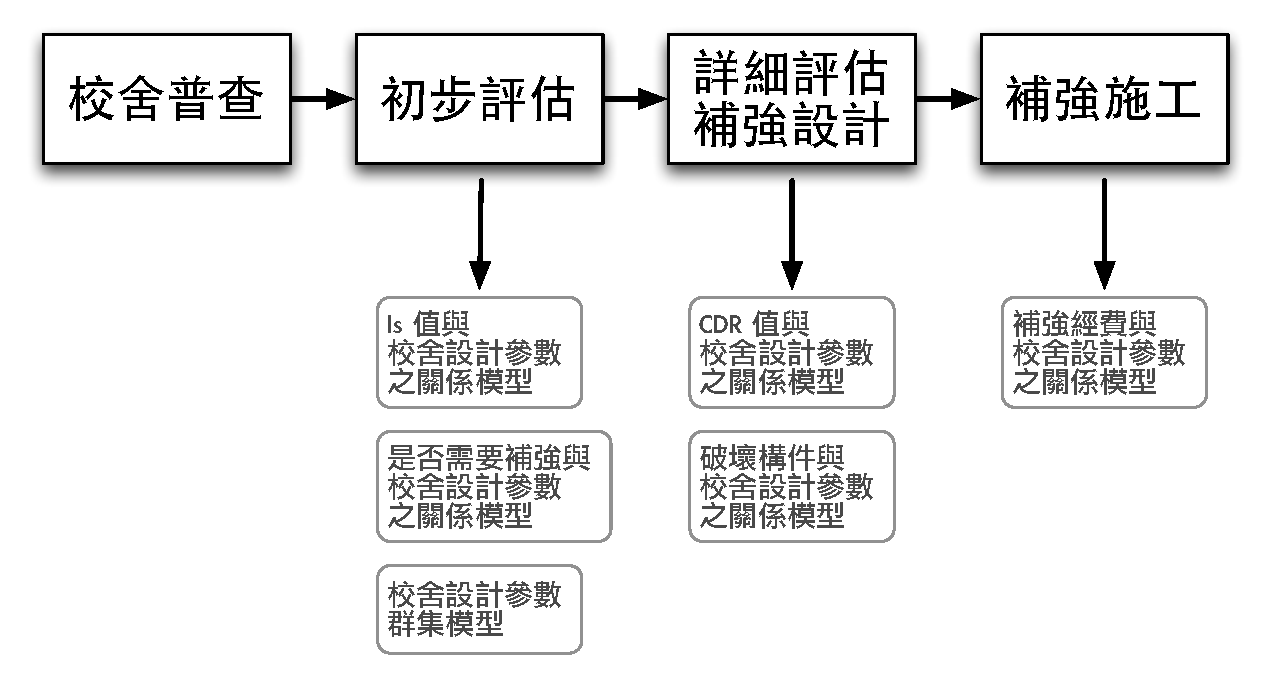
\includegraphics[width=1.0\textwidth]{figures/survey-flow-con.pdf}
    \caption{評估流程與資料探勘模型} 
    \label{fig:FLOW-con}
  \end{center}
\end{figure}

本研究所提出數個基於校舍耐震資料庫與資料探勘方法所得到的關係模型,均有不錯的表現,而這些關係模型的目標屬性均是校舍耐震能力補強計畫的工作流程中,不同階段的產出,透過這些關係模型,可以快速的得到本來是非線性關係,不容易取得的關鍵屬性,並且保有一定程度的可靠性,這些模型雖然無法直接的取代現有的評估流程,但是其知識之內容相信可以輔助整個校舍耐震能力補強計畫的工作,例如:藉由~$Is$~值的關係模型來判斷一群校舍整體的耐震能力表現、甚至是可以直接使用補強經費得關係模型來輔助決策者,判斷要編列多少預算,並且可以同時瞭解到這些預算可以完成多少校舍的補強、這些校舍佔所有耐震能力有疑慮的校舍中的比例,甚至是反過來,根據決策者決定要補強多少棟或是多少比例的校舍,再透過關係模型計算這些校舍的總補強經費為多少,提供給決策者做參考。這些應用都可以有效的提升校舍耐震能力補強作業的效能,讓主事者更快的瞭解校舍的狀況,並且更有效的分配預算。

\section{未來展望} 

本論文目前之主要之成果為耐震能力與補強預算相關之知識,然而本研究初期時即依照資料探勘的四種知識類型:迴歸、分類、分群、關聯分別分析設計了數個不同面像的探勘目標如圖~\ref{fig:bigpicture}~,分別詳述如下:

\begin{description}
  \item[迴歸]
  主要的知識為重要屬性的關係模型,且要為數值類型的屬性,例如校舍的最小破壞地表加速度、耐震能力、補強經費等。
  \item[分類]
  分類探勘類型的知識和迴歸類之知識相似,主要也是用在建立重要屬性的關係模型,其主要差異在於迴歸分析僅能對數值類型之屬性建立模型,而分類分析則僅能對資料數值為集合類之屬性建立模型,目前所設計之分析為校舍是否安全、是否需要補強的分類分析。
  \item[分群]
  分群類型之知識主要在於校舍結構之不同群集,其知識之形式與分類分析有些相似,最大之不同點在於此類模型在訓練建立時,並沒有輸出參數,而是只靠輸入參數間來判斷資料間的相似度,例如相似結構形式的校舍群集,組成校舍的結構元件的探勘等。
  \item[關聯]
  此類型之知識形式為屬性間的特殊關係,例如特定年代的校舍在設計上會有不同於其他年代的的形式,而這些特色如果可以在典型校舍的設計參數上表現出來,應當可以用此種資料探勘尋找出來,而預期的目標包括了不同年代校舍之設計特色、校舍結構之設計模式等。
\end{description}

\begin{figure}[hbtp]
  \begin{center}
    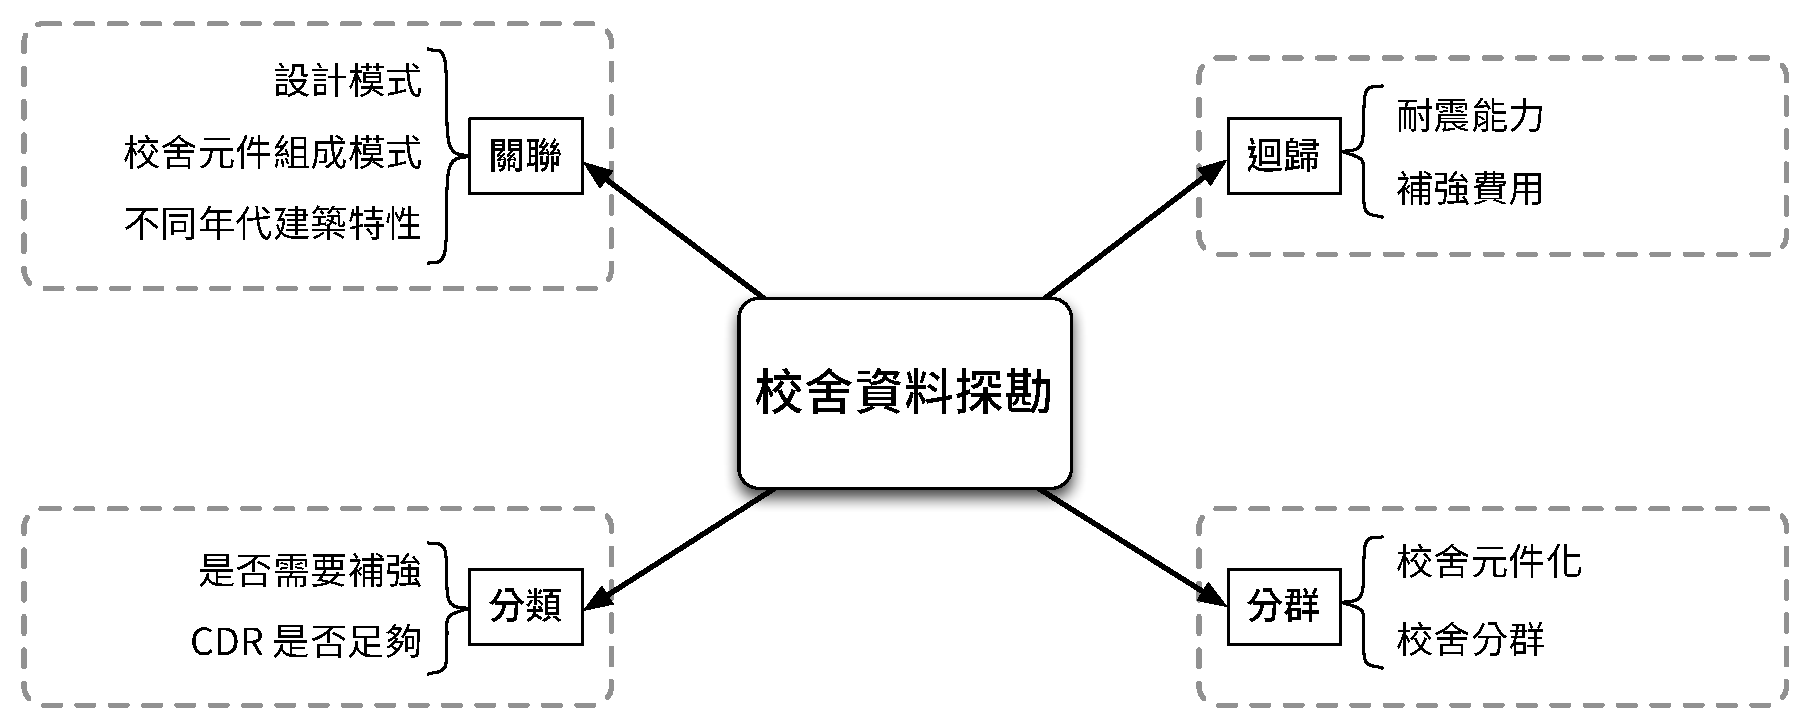
\includegraphics[width=1.0\textwidth]{figures/big-picture.pdf}
    \caption{知識挖掘規劃} 
    \label{fig:bigpicture}
  \end{center}
\end{figure}

本研究目前透過資料探勘所得到之知識,均分佈在教育部的校舍耐震能力補強的流程之上,包括了分類形式的校舍是否需要補強與其設計參數之關係模型、迴歸形式的校舍耐震能力與其設計參數之關係模型以及校舍補強經費與其設計參數之關係模型、還有分群形式的校舍群集模型,其在建立耐震能力關係模型時,作為資料前處理輔助用。而第一個發展方向,就是更進一步往不同的方向進行資料探勘,例如初期規劃所設計的探勘目標,在關聯形式的知識尚沒有任何可用的成果,但是研究初期規劃的那些知識隱含於耐震資料庫中的可能性極高,而且這類知識的發掘雖然無法直接回饋到校舍耐震補強計畫之上,但是卻可能在其它的校舍相關議題上發揮其功用。

% 主要都是以輔助目前的校舍耐震能力補強計畫流程作為出發點

% 在本研究中,建立校舍設計參數與其~$Is$~值之關係模型時,便有使用到此一知識來增進關係模型的品質,後續研究還可以針對這些校舍群集,進一步分析其不同群集之特性,至於關聯形式的知識,本研究目前尚未有可用的知識產出,因此後續的研究方向也包含此一類型知識的探勘與挖掘。

第二個發展方向,則是可以嘗試將目前獨立分佈在耐震能力補強流程上的數個資料探勘也串接起來,由於目前資料的複雜度的關係問題,不同的資料探勘分析都是獨立進行分析,包括資料前處理的資料篩選也是根據問題的特性來調整,因此不同的模型所需要的輸入資料的屬性,雖然有很大程度是相關的屬性,但是仍有吃易,也造成判斷校舍是否需要補強的的輸入資料集無法用作~$CDR$~值關係模型的輸入之用,$CDR$~值關係模型的輸入資料集也無法用作補強經費關係模型的輸入之用。但是也因為不同模型的輸入資料屬性有很大的相關度,那也表示應該可以探討出一組資料屬性集,同時可以找出和初步評估的~$Is$~值關係模型、詳細評估的~$CDR$~值以及補強校舍的補強經費都能夠找出其關係模型,那麼應該可以用這組模型,在校舍建築物調查非常初始的階段,就能夠推估它的耐震能力表現如何、是否足夠,進一步到是否需要補強、補強經費多少。

最後一個發展方向,則是在~CRISP-DM~流程當中的最後一個步驟,將探勘得到的知識實際回饋到學校校舍及相關設備補強整建計畫上,由於目前探勘得到的知識都還是以數學模型的形式存在,非專業人士難以應用,因此如果可以將這些數學模型轉化成決策支援系統,則可以讓主管機關能夠簡單的得到這些模型的輔助,在校舍長期持續的耐震能力監控上,能夠發揮探勘所得知識的效力。







	%----------------------------------------------------------------------------------------------------------------------------------------------------------
	% back pages 後頁
	% 包括參考文獻、附錄、自傳
	% 實際內容由
	%    my_bib.bib, my_appendix.tex, my_vita.tex
	% 決定
	% ntust_backpages.tex 此檔只提供整體架構的定義,不需更動
	% 在撰寫各章草稿時,可以把此部份「關掉」,以節省無謂的編譯時間。
	%\bibliographystyle{unsrt} 
	%
% this file is encoded in utf-8
% v1.7

%%% 參考文獻
\newpage
%\bibliographystyle{unsrt}
\cleardoublepage
\phantomsection
\addcontentsline{toc}{chapter}{\nameRef}
\renewcommand{\bibname}{\protect\makebox[5cm][s]{\nameRef}}
%  \makebox{} is fragile; need protect
%\bibliographystyle{unsrt} 
\bibliographystyle{ieeetr}  % 使用 IEEE Trans 期刊格式
%\bibliographystyle{unsrt}
\bibliography{my_bib}  %reference 所需的bib檔
%\bibliographystyle{unsrt} 

%%% 附錄
%
% this file is encoded in utf-8
% v1.7
%%% 每一個附錄 (附錄一、附錄二、...) 都要複製此段附錄編排碼做為起頭
%%% 附錄編排碼 begin >>>

\includepdfset{pages=-,pagecommand=\thispagestyle{AppendixPage}}

\newpage
\chapter*{附錄一:典型校舍初步評估表} % 修改附錄編號與你的附錄名
\label{appendix-pe}
\addcontentsline{toc}{chapter}{附錄一:典型校舍初步評估表} %建議此內容應與上行相同
\renewcommand{\thechapter}{一} % 如果是附錄二,則內容應為{二}

\setcounter{equation}{0} 
\setcounter{figure}{0} 
\setcounter{footnote}{0} 
\setcounter{section}{0} 
\setcounter{subsection}{0}
\setcounter{subsubsection}{0}
\setcounter{table}{0} 
%%% <<< 附錄編排碼 end

% 附錄內容開始
見下頁。

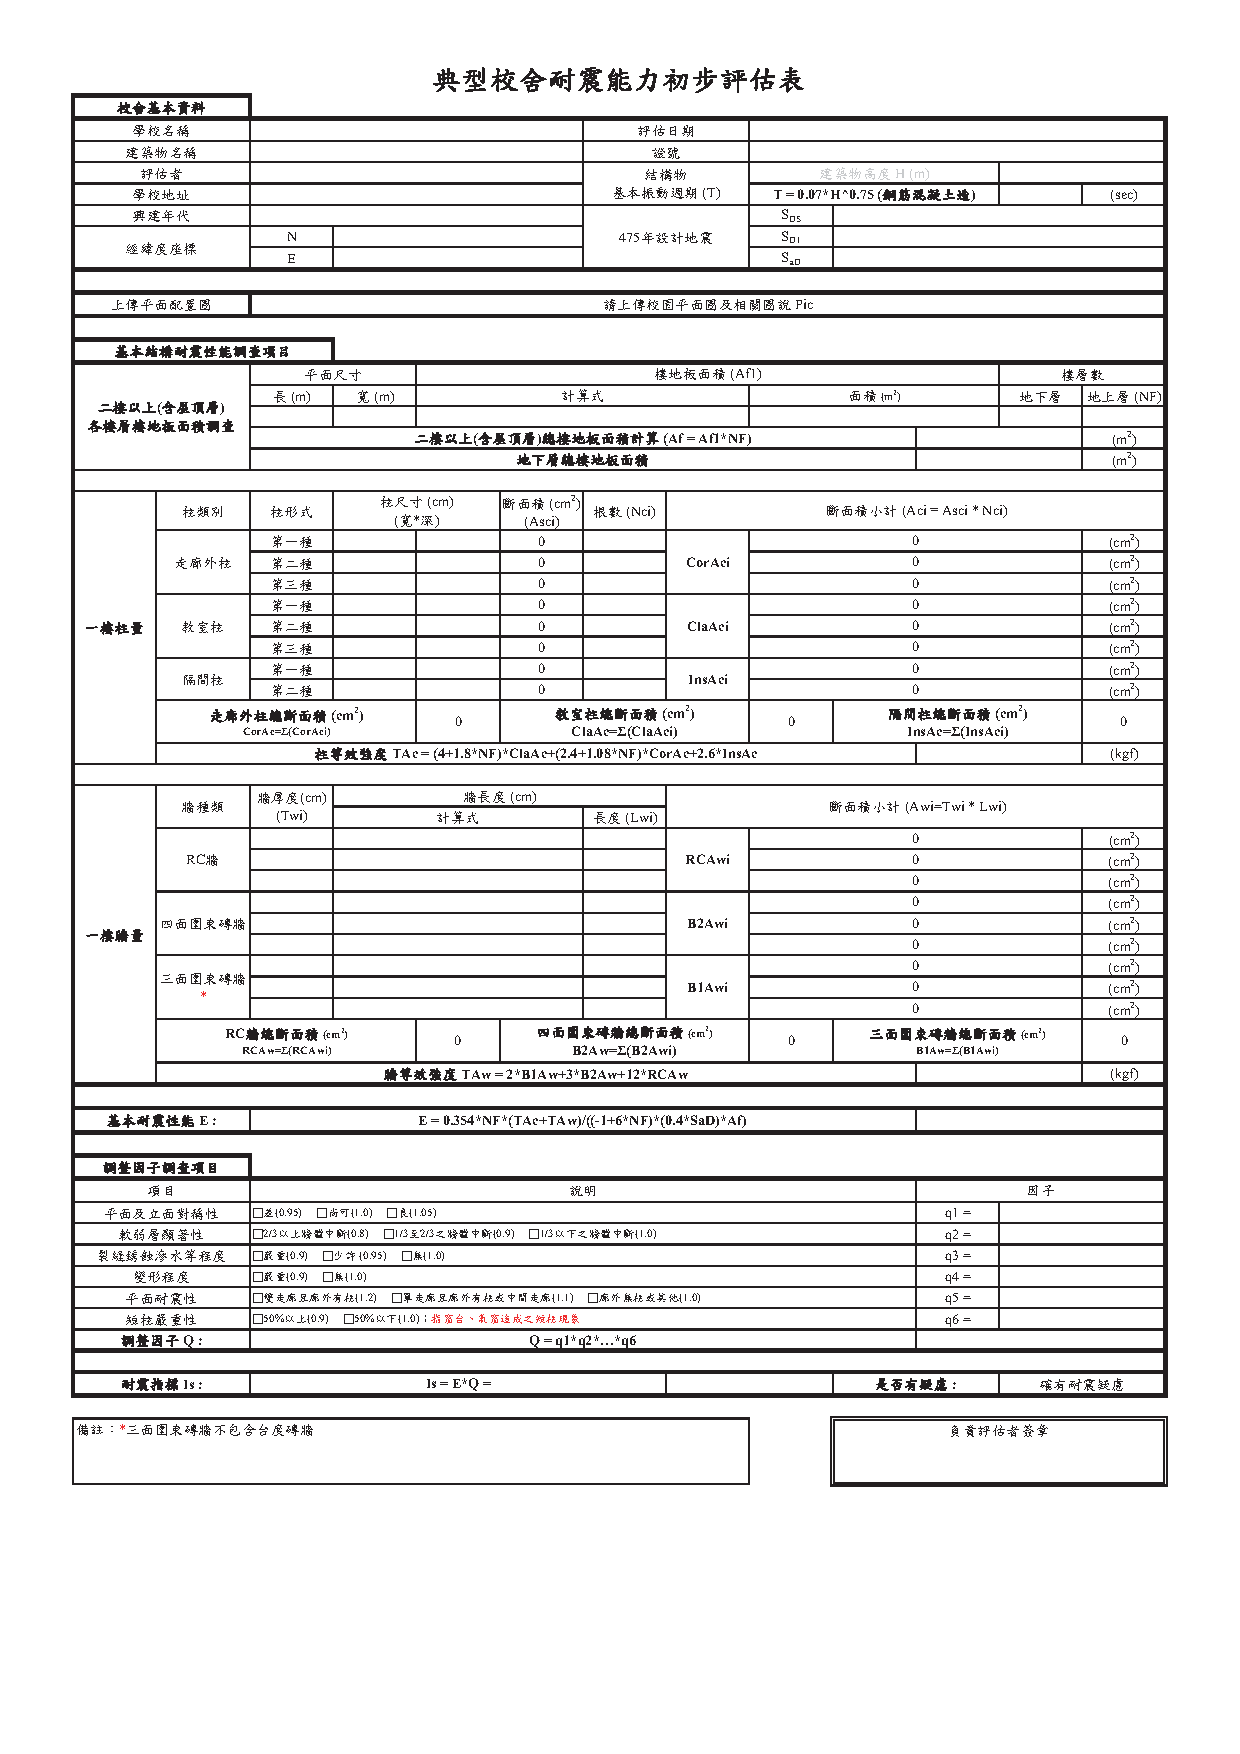
\includepdf[fitpaper=true,scale=0.95]{appendix/20120516-Preliminary-Typical.pdf}

%%% 如果有附錄二、三、...,則在此繼續加上「附錄編排」碼
% 每一個附錄會自動以新頁開始

\newpage
\chapter*{附錄二:典型校舍詳細評估表} % 修改附錄編號與你的附錄名
\label{appendix-de}
\addcontentsline{toc}{chapter}{附錄二:典型校舍詳細評估表} %建議此內容應與上行相同
\renewcommand{\thechapter}{二} % 如果是附錄二,則內容應為{二}

\setcounter{equation}{0} 
\setcounter{figure}{0} 
\setcounter{footnote}{0} 
\setcounter{section}{0} 
\setcounter{subsection}{0}
\setcounter{subsubsection}{0}
\setcounter{table}{0} 
%%% <<< 附錄編排碼 end

% 附錄內容開始
見下頁。


\includepdf[fitpaper=true,scale=0.95]{appendix/detailed-evaluation.pdf}


\newpage
\chapter*{附錄三:典型校舍補強設計表} % 修改附錄編號與你的附錄名
\label{appendix-re}
\addcontentsline{toc}{chapter}{附錄三:典型校舍補強設計表} %建議此內容應與上行相同
\renewcommand{\thechapter}{三} % 如果是附錄二,則內容應為{二}

\setcounter{equation}{0} 
\setcounter{figure}{0} 
\setcounter{footnote}{0} 
\setcounter{section}{0} 
\setcounter{subsection}{0}
\setcounter{subsubsection}{0}
\setcounter{table}{0} 
%%% <<< 附錄編排碼 end

% 附錄內容開始
見下頁。

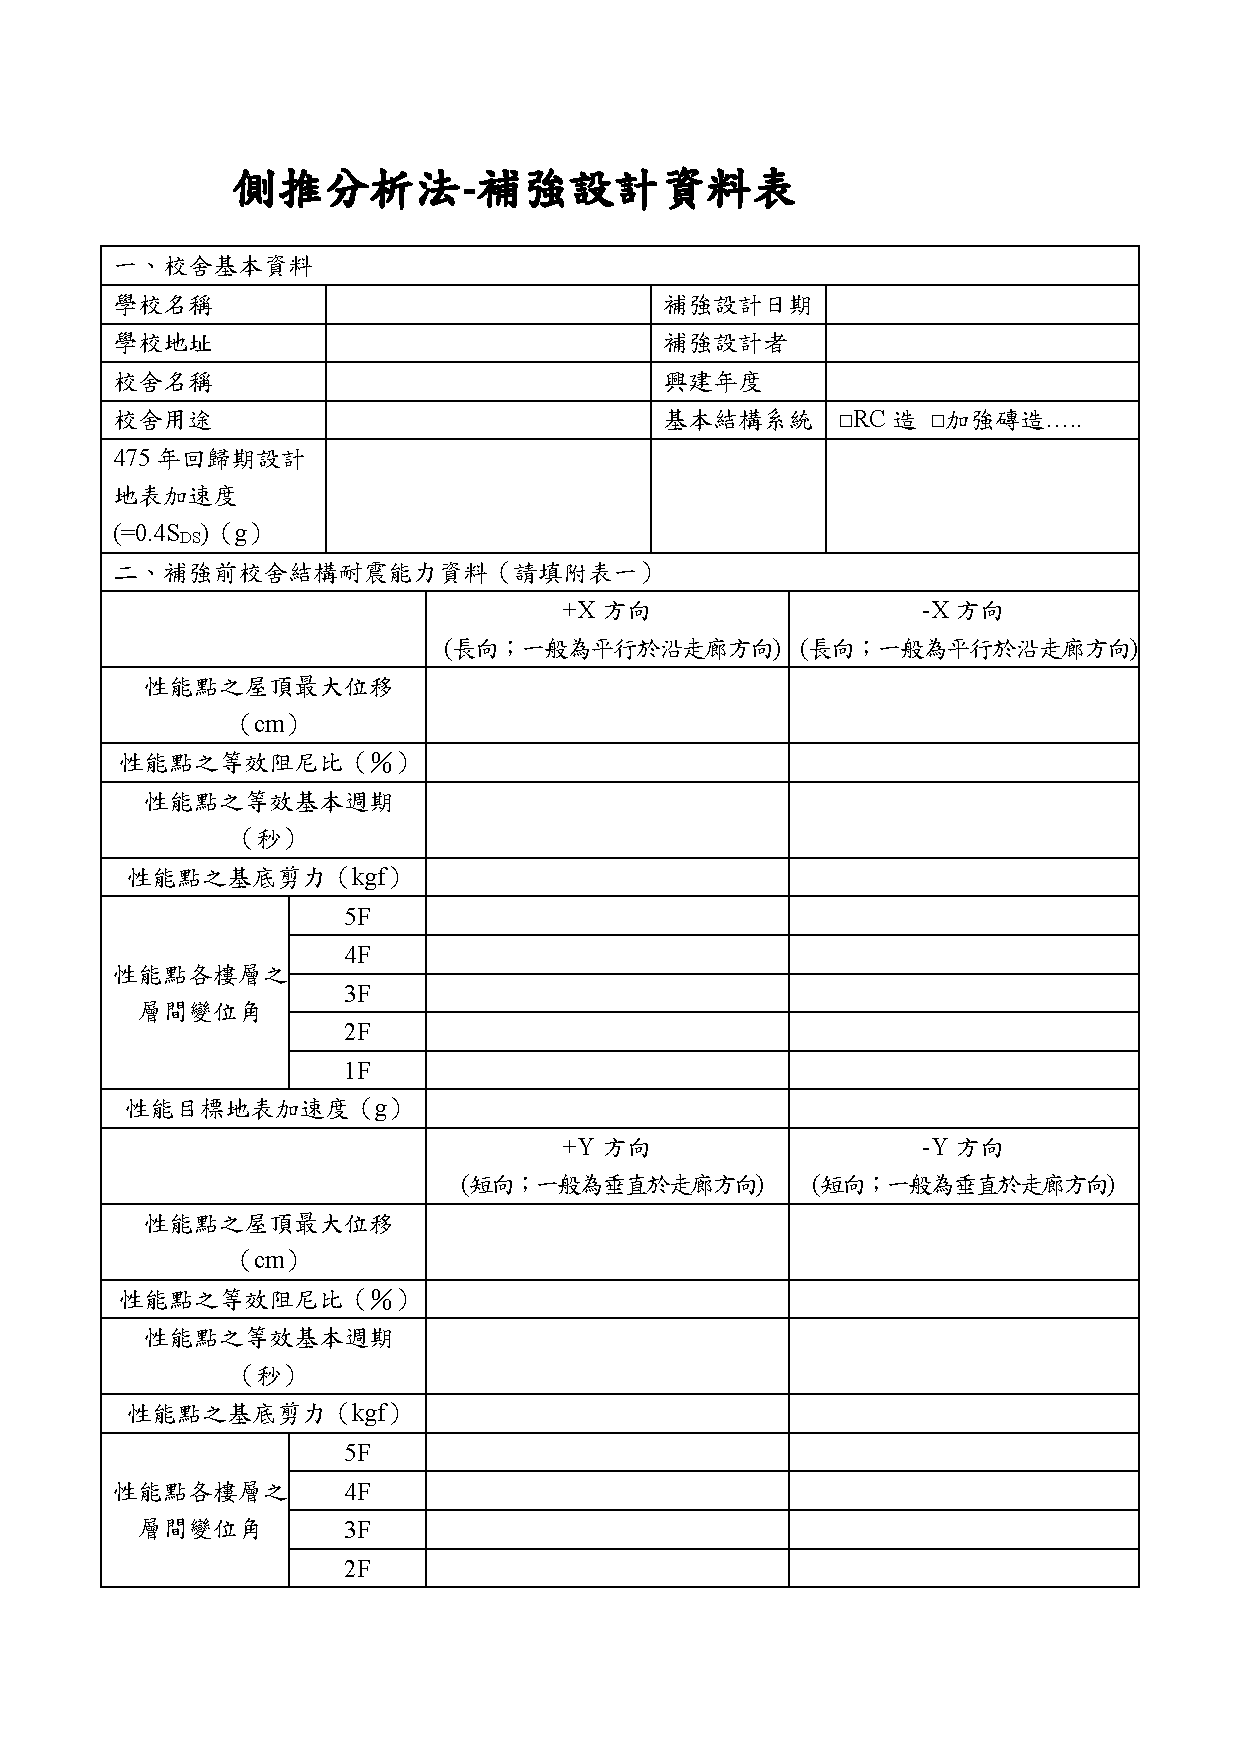
\includepdf[fitpaper=true,scale=0.95]{appendix/retrofit.pdf}

%%% 自傳
%\newpage
%\chapter*{\protect\makebox[5cm][s]{\nameVita}} % \makebox{} is fragile; need protect
%\addcontentsline{toc}{chapter}{\nameVita}
%本人生於 1981 年 1 月 1 日,在桃園內壢。家裡經營電器行,上有一位姊姊。從小就喜歡拆解店裡收回的報廢家電用品,練就了一身好手藝與探究一切的好奇心。

國小就讀平鎮國小。由於把供應全校用水的抽水馬達拆開研究裝不回去,造成全校停水,廁所污穢不堪。被校長處罰掃廁所一個星期。那真是我少時年幼無知的一頁插曲。



%%%%%%%%%%%%%%%%%%%%%%%%%%%%%%%
%       授權書 (計頁碼,但不印頁碼) 
%%%%%%%%%%%%%%%%%%%%%%%%%%%%%%%
%
% insert the printed standard form when the thesis is ready to bind
% 在口試完成後,再將已簽名的授權書放入以便裝訂
% create an entry in table of contents for 授權書
% 目前送出空白頁
\cleardoublepage
\phantomsection
%
\includepdf[fitpaper=true,scale=1,pagecommand=\thispagestyle{empty}]{backpages/G-15.pdf}

\includepdf[fitpaper=true,scale=1,angle=90,pagecommand=\thispagestyle{empty}]{backpages/img-122151637-0001.pdf}


	%\bibliographystyle{unsrt} 



\end{document} 
 
